\documentclass[9pt, draft]{beamer}

\usepackage{appendixnumberbeamer}
\usepackage{booktabs}
\usepackage[scale=2]{ccicons}
\usepackage{pgfplots}
% \usepackage{tikz}
\usepackage{circuitikz}
\usepackage{graphics}
\usepackage{soul}

\usepgfplotslibrary{dateplot}
\pdfstringdefDisableCommands{\def\translate#1{#1}}
\geometry{paperwidth=140mm, paperheight=105mm}
\usetheme{metropolis}
\bibliographystyle{abbrv}
\setbeamertemplate{frame footer}{Metamaterials and Metastructures}

\usetikzlibrary{shapes, arrows}
\tikzstyle{startstop} = [rectangle, rounded corners, minimum width=2cm, minimum height=1cm, text centered, draw=black, fill=red!30]
\tikzstyle{io} = [trapezium, trapezium stretches=true, trapezium left angle=70, trapezium right angle=110, minimum width=2cm, minimum height=1cm, text centered, draw=black, fill=blue!30]
\tikzstyle{process} = [rectangle, minimum width=2cm, minimum height=1cm, text centered, text width=2cm, draw=black, fill=orange!30]
\tikzstyle{decision} = [diamond, minimum width=2cm, minimum height=1cm, text centered, draw=black, fill=green!30]
\tikzstyle{arrow} = [thick,->,>=stealth]

\title{Study on Nonreciprocal Behavior in Time-Space Modulated Beams}
\subtitle{Control of structural band-gaps via shunted piezoelectric patches}
\date{12/02/2025}
\author{Tommaso Bocchietti 10740309 \\ Konstantinos Georgoussis 10992540 \\ (Luciano Sarri 11071336)}
\institute{Politecnico di Milano}
\titlegraphic{\hfill
\includegraphics[height=1.5cm]{pdf/Polimi_logo_header.pdf}}

\begin{document}

\maketitle

\begin{frame}{Agenda}

    \begin{columns}[c, onlytextwidth]

        \begin{column}{0.4\textwidth}

            \setbeamertemplate{section in toc}[sections numbered]
            \tableofcontents

        \end{column}

        \begin{column}{0.6\textwidth}

            \begin{figure}[H]
                \centering
                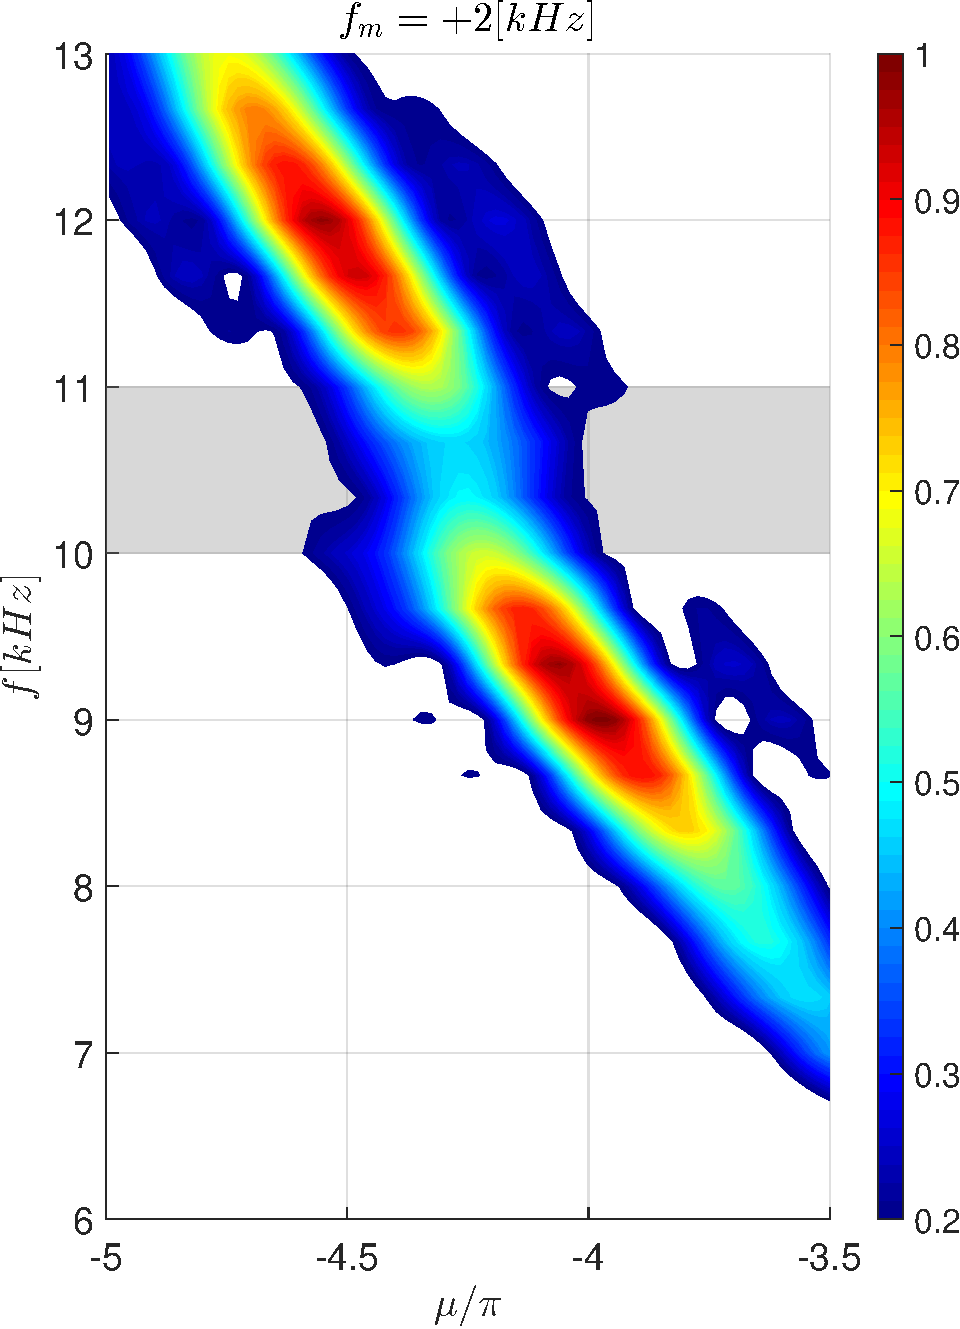
\includegraphics[width=0.47\textwidth]{img/MATLAB/EXP_nonreciprocal_@+2kHz.pdf}
                \hspace{1mm}
                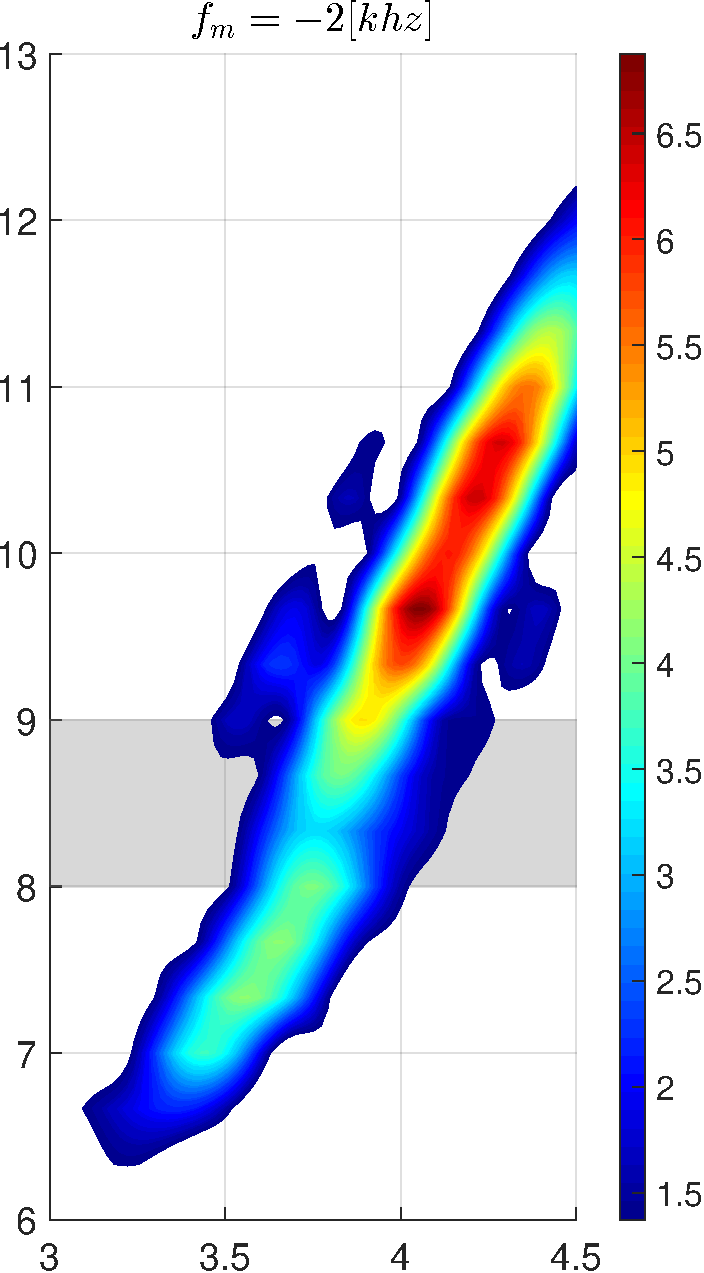
\includegraphics[width=0.47\textwidth]{img/MATLAB/EXP_nonreciprocal_@-2kHz.pdf}
                \caption{Experimental results of nonreciprocal behavior.}
            \end{figure}

        \end{column}

    \end{columns}

\end{frame}

\section{Introduction}


\begin{frame}{Introduction to nonreciprocity}

    The principle of reciprocity states that the in a linear time-invariant system (LTI), waves propagate from $A$ to $B$ in the same way as from $B$ to $A$.
    The violation of this principle is referred to as \textbf{nonreciprocal} behavior.

    \vspace{9pt}

    One question arise: \textbf{is it possible to design a system that achieves nonreciprocal behavior?}

    % Breaking reciprocity in wave propagation enables the development of one-way communication devices with enhanced performance.

\end{frame}



\begin{frame}{Experimental setup}

    The experimental setup\footnotemark[1] is composed of an array of shunted piezoelectric patches spaced $2$ mm apart placed on an aluminum beam substrate.
    Toggling the switches that control the connection between the power supply and each negative capacitance shunting circuit, allows to modulate the substrate properties.

    \begin{figure}[H]
        \centering
        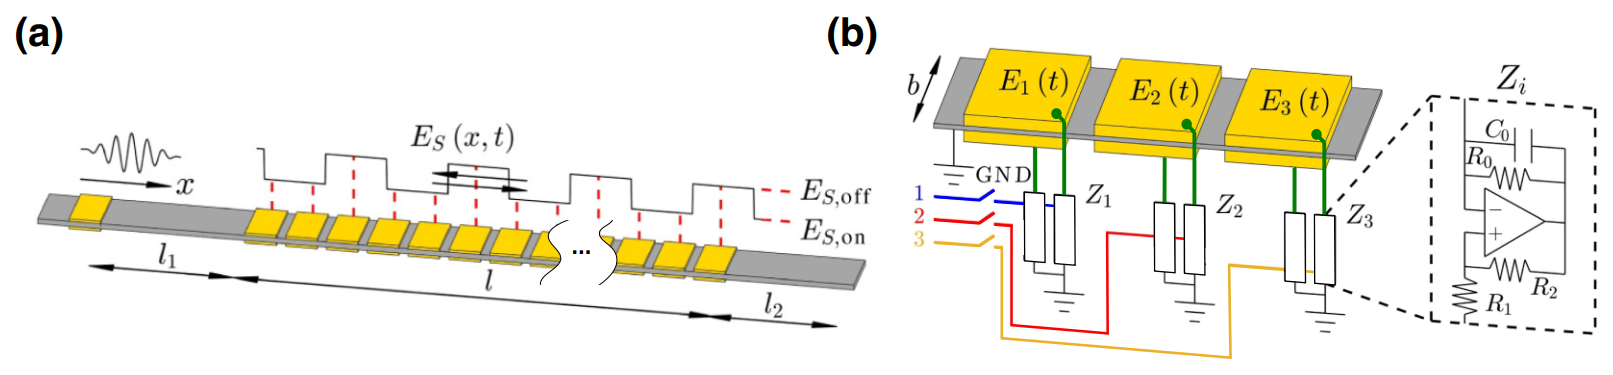
\includegraphics[width=0.9\textwidth]{img/experimental_setup_scheme.png}
        \caption{Beam substrate and array of piezoelectric patches (a), Spatio-Temporal cell and shunting circuits (b).}
    \end{figure}

    Out-of-plane velocity field is measured using a Polytec 3D laser Doppler vibrometer.

    \footnotetext[1]{For numerical values and detailed description, refer to the attached project report (Section 4.1).}

\end{frame}



\begin{frame}{Experimental setup}

    By connecting the piezoelectric patches to the beam, the effective properties of the system are modified.

    \vspace{9pt}

    \begin{columns}[c, onlytextwidth]

        \begin{column}{0.6\textwidth}

            \begin{figure}[H]

                \centering

                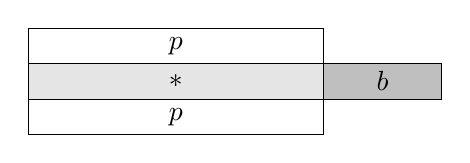
\begin{tikzpicture}[scale=1.5]

                    % Beam
                    \draw[fill=gray!20] (0,0) rectangle (2.5,0.3) node[midway] {$*$};
                    \draw[fill=gray!50] (2.5,0) rectangle (3.5,0.3) node[midway] {$b$};

                    % Piezoelectric patches
                    \draw[fill=white] (0, 0.3) rectangle (2.5, 0.6) node[midway] {$p$};
                    \draw[fill=white] (0, 0.0) rectangle (2.5, -0.3) node[midway] {$p$};

                \end{tikzpicture}

                \caption{Connection between piezoelectric patches and beam.}

            \end{figure}

        \end{column}

        \begin{column}{0.4\textwidth}

            \begin{equation}
                \begin{aligned}
                    EJ^*     & = E_b J_b + 2 E_p J_p       \\
                    \rho A^* & = \rho_b A_b + 2 \rho_p A_p
                \end{aligned}
            \end{equation}

        \end{column}

    \end{columns}

\end{frame}
\section[Analysis of shunted piezoelectric patches]{Shunted piezoelectric patches}

\begin{frame}{Piezoelectric patches sensitivity to $RLC_N$ shunting circuit}

    \begin{columns}[c, onlytextwidth]

        \begin{column}{0.3\textwidth}

            \begin{figure}[H]

                \centering

                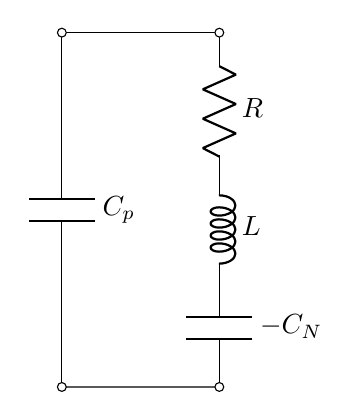
\begin{tikzpicture}[european voltages]

                    % Upper and lower horizontal lines
                    \draw (0,0) to [short] ++(2,0);
                    \draw (0,-4.5) to [short] ++(2,0);

                    % Piezo
                    \draw (0,0) to [C, l=$C_p$, o-o] ++(0,-4.5);

                    % Shunt
                    \draw (2,0)
                    to [R, l=$R$, o-] ++(0,-2)
                    to [L, l=$L$] ++(0,-1)
                    to [C, l=$-C_N$, -o] ++(0,-1.5);

                \end{tikzpicture}

                \caption{$RLC_N$ shunting circuit}

            \end{figure}

        \end{column}

        \hfill

        \begin{column}{0.65\textwidth}

            \textbf{The mechanical admittance of piezoelectric patches is influenced by the presence of shunting circuits}:

            \begin{equation}
                \begin{aligned}
                    Y^{SU} & = Y_1^D \left( 1 - \frac{k_{31}^2}{1 + s C_p^S Z^{SU}} \right)                                               \\
                           & = Y_1^D \left( 1 - \frac{k_{31}^2}{1 + C_p^S \left( -\frac{1}{C_N} - \omega^2 L \right) - s C_p^S R} \right)
                \end{aligned}
                \label{eq:Y_SU_RLC_N}
            \end{equation}

            \vspace{9pt}

            Negative capacitance ($-C_N < 0$) are active elements that can be implemented via OP-AMPs.
            As active elements, stability analysis is required:

            \begin{itemize}
                \item Mechanically stable if $Y^{SU} > 0$;
                \item Electrically stable if $C_{tot} > 0$.
            \end{itemize}

        \end{column}

    \end{columns}

    \vspace{9pt}

    A complete sensitivity analysis of $Y^{SU}(Z^{SU})$ is shown in the next slides.

\end{frame}



\begin{frame}{Short vs. Open circuit case}

    \begin{figure}[H]
        \centering
        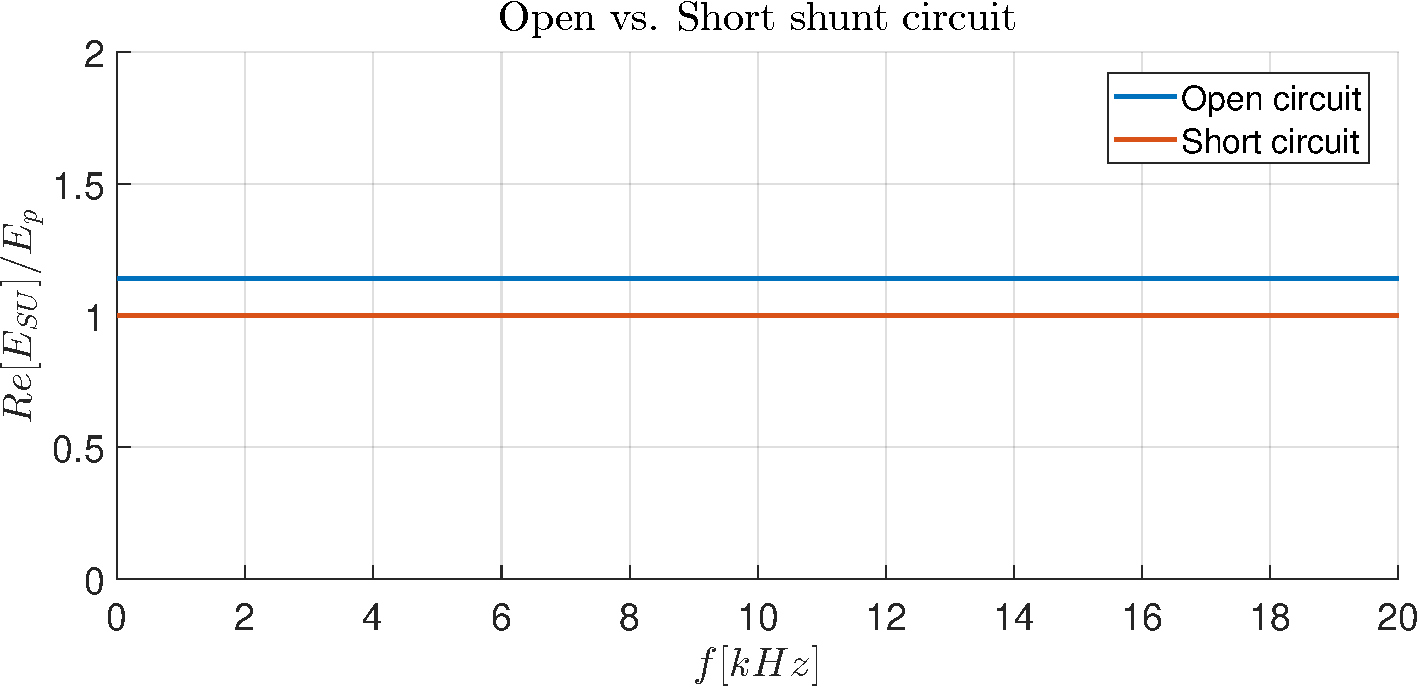
\includegraphics[width=0.7\textwidth]{./img/MATLAB/Y_SU_Open vs Short circuit.pdf}
        \caption{Analysis of $Y^{SU}$ for the open and short circuit case.}
    \end{figure}

    As predicted by Equation \ref{eq:Y_SU_RLC_N}, the piezoelectric patches' mechanical admittance in case of open circuit is greater than in case of short circuit.
    This causes a stiffer substrate and indeed a shift of the band-gap towards higher frequencies.

    \begin{equation}
        Y_1^D > Y_1^E = Y_1^D (1 - k_{31}^2)
    \end{equation}

\end{frame}



\begin{frame}{Short vs. Open circuit case}


    \only<1-2>{

        \begin{figure}[H]
            \centering
            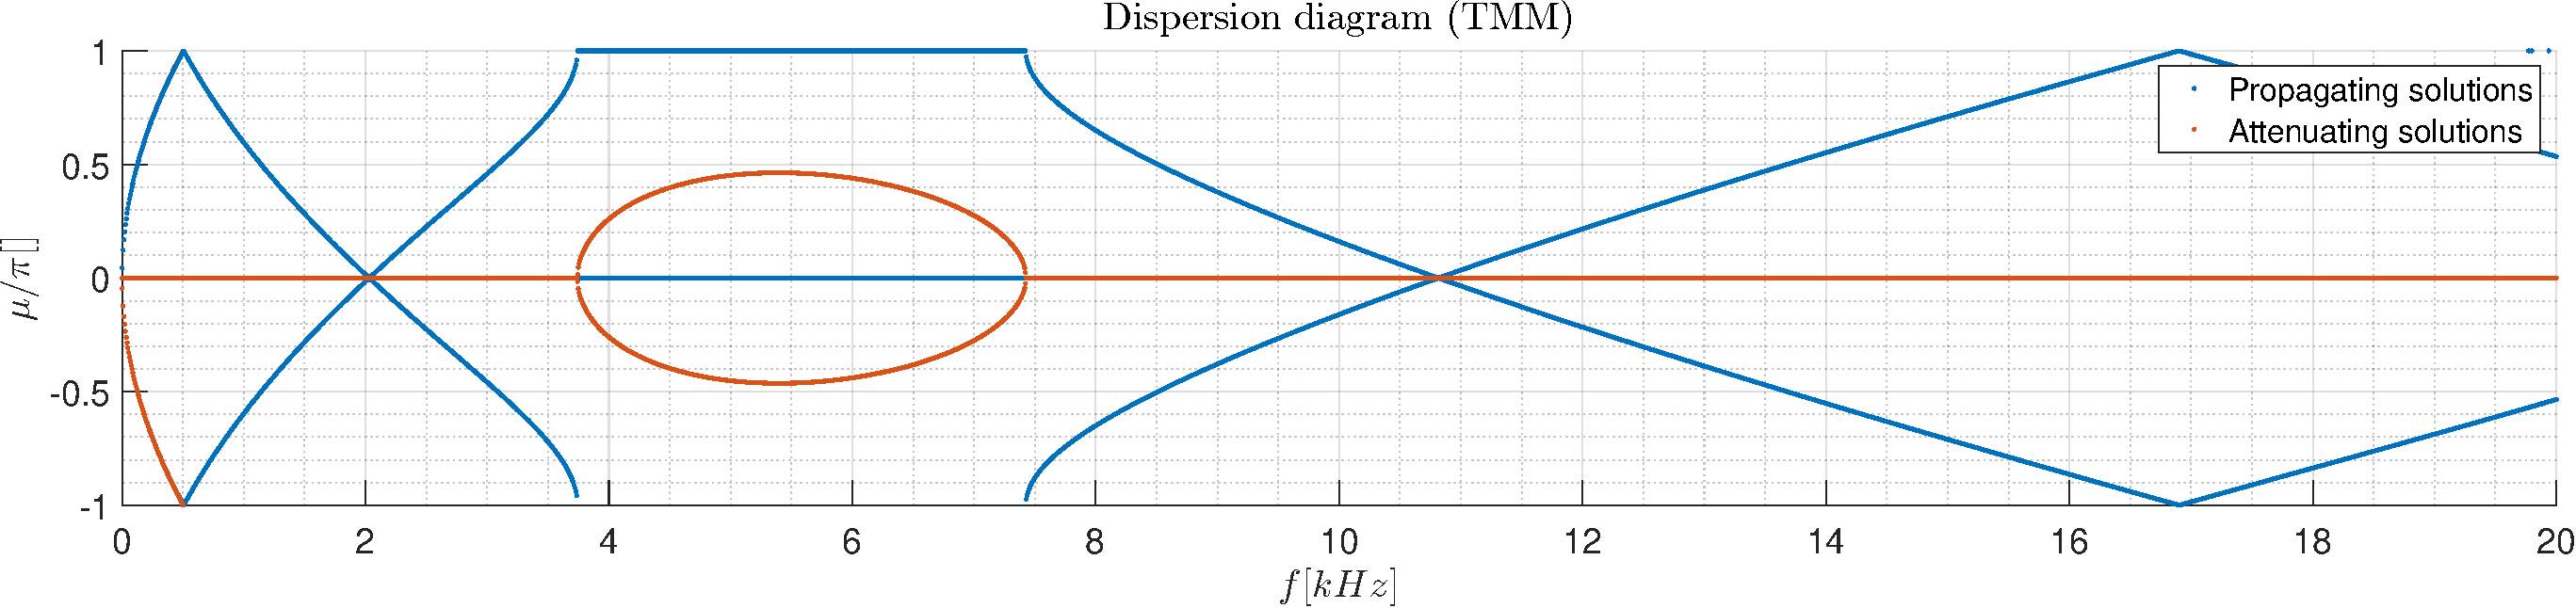
\includegraphics[width=\textwidth]{./img/MATLAB/TMM_ON-ON-ON_OFF_R1000_L0.015_C5e-09.pdf}
            \caption{Short circuit case.}
        \end{figure}

    }

    \only<2->{

        \begin{figure}[H]
            \centering
            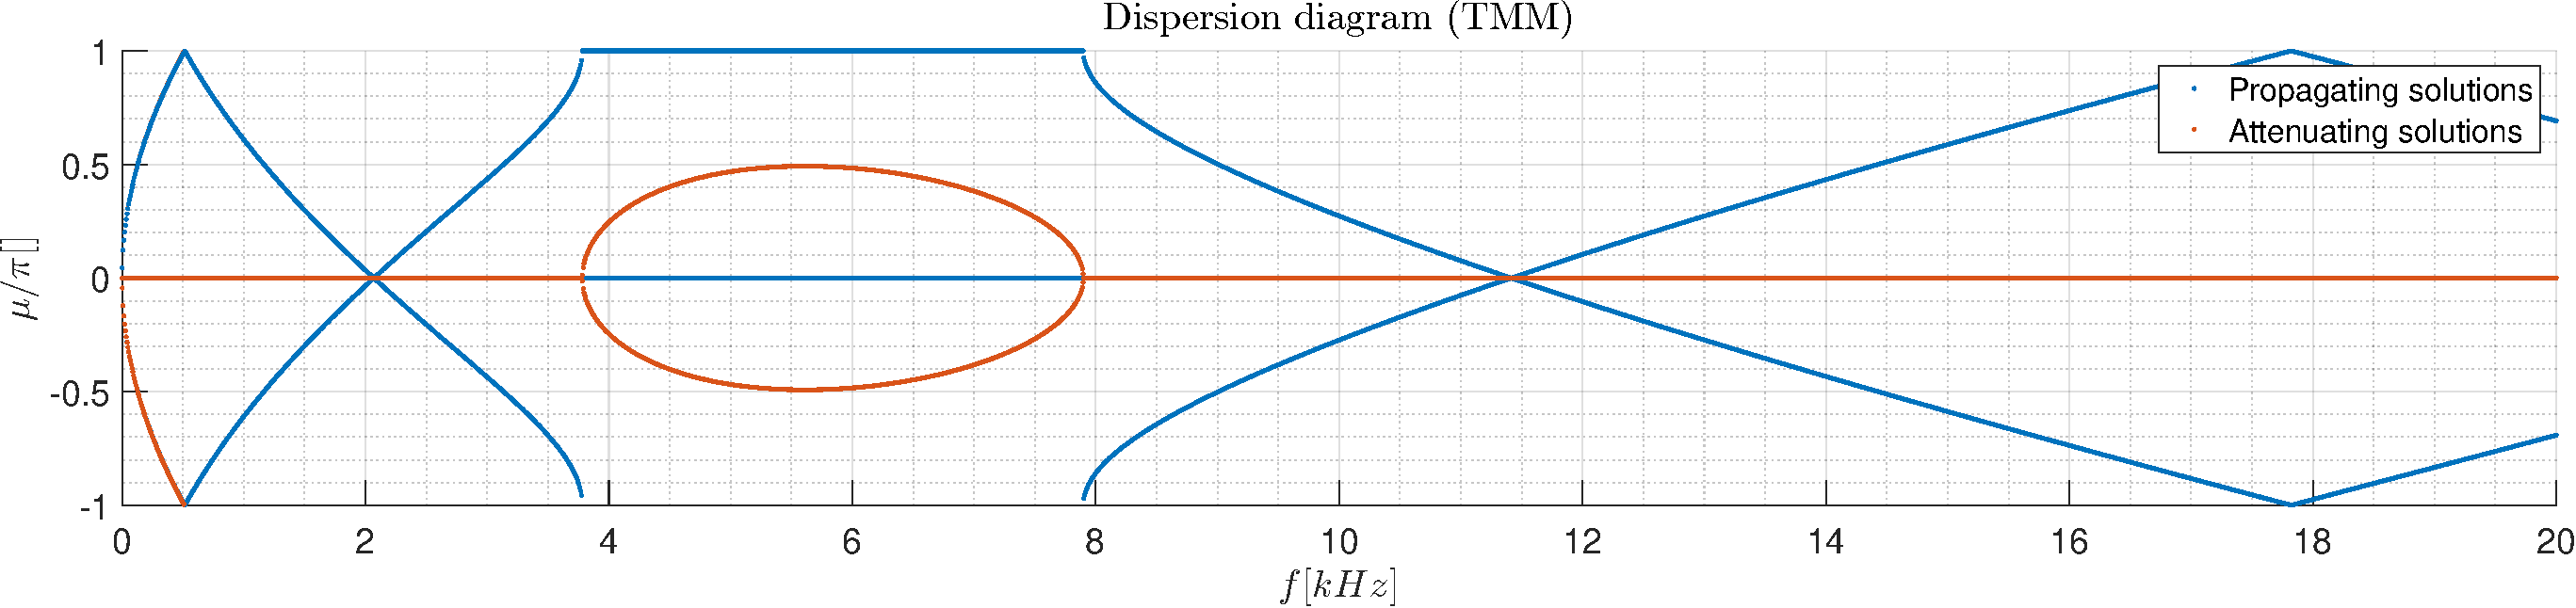
\includegraphics[width=\textwidth]{./img/MATLAB/TMM_ON-ON-ON_+inf_R1000_L0.015_C5e-09.pdf}
            \caption{Open circuit case.}
        \end{figure}

    }

\end{frame}



\begin{frame}{$L$ shunt circuit}

    \begin{figure}[H]
        \centering
        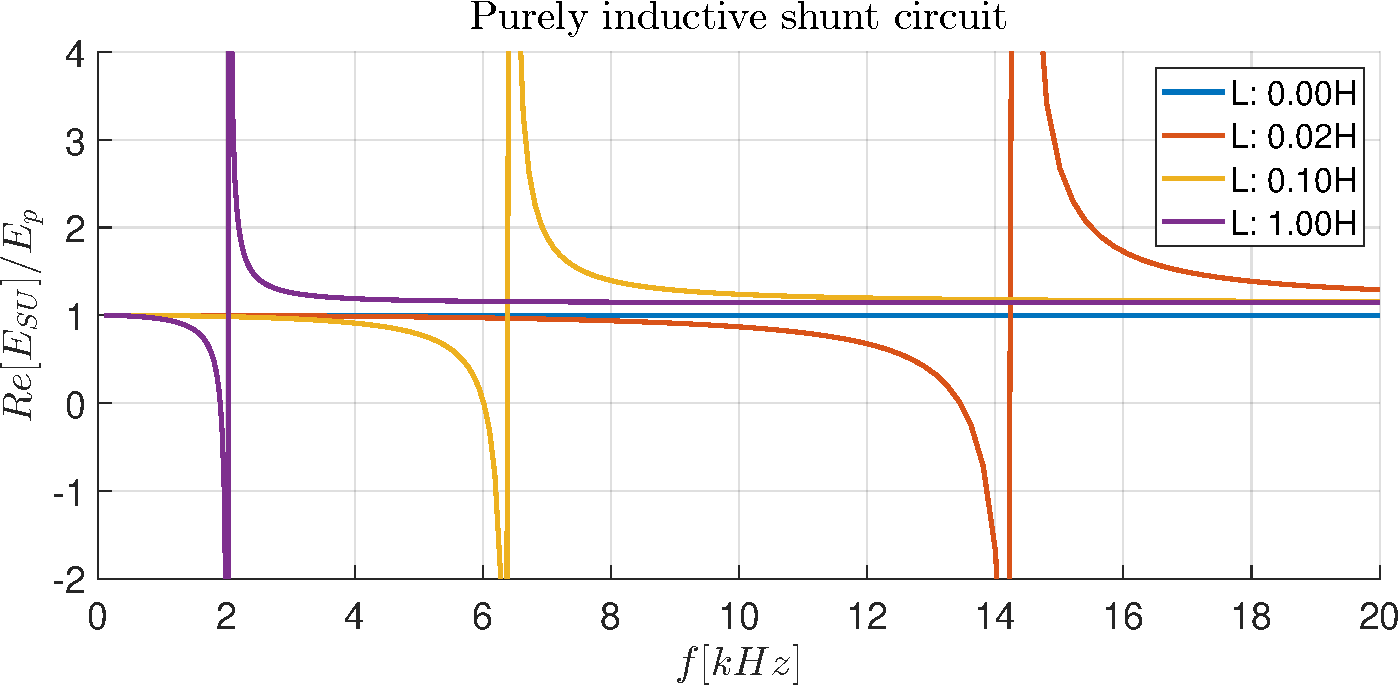
\includegraphics[width=0.7\textwidth]{./img/MATLAB/Y_SU_Purely inductive shunt circuit.pdf}
        \caption{Analysis of $Y^{SU}$ for the purely inductive shunt circuit.}
    \end{figure}

    In case of $L$ shunt circuit, mechanical admittance of the piezoelectric patches is given by:

    \begin{equation}
        Y^{SU} = Y_1^D \left( 1 - \frac{k_{31}^2}{1 -\omega^2 C_p^S L} \right)
    \end{equation}

    Oscillatory behavior is expected around the natural frequency $\omega_n = \frac{1}{\sqrt{C_p^S L}}$.

\end{frame}



\begin{frame}{$L$ shunt circuit}

    \only<1-2>{

        \begin{figure}[H]
            \centering
            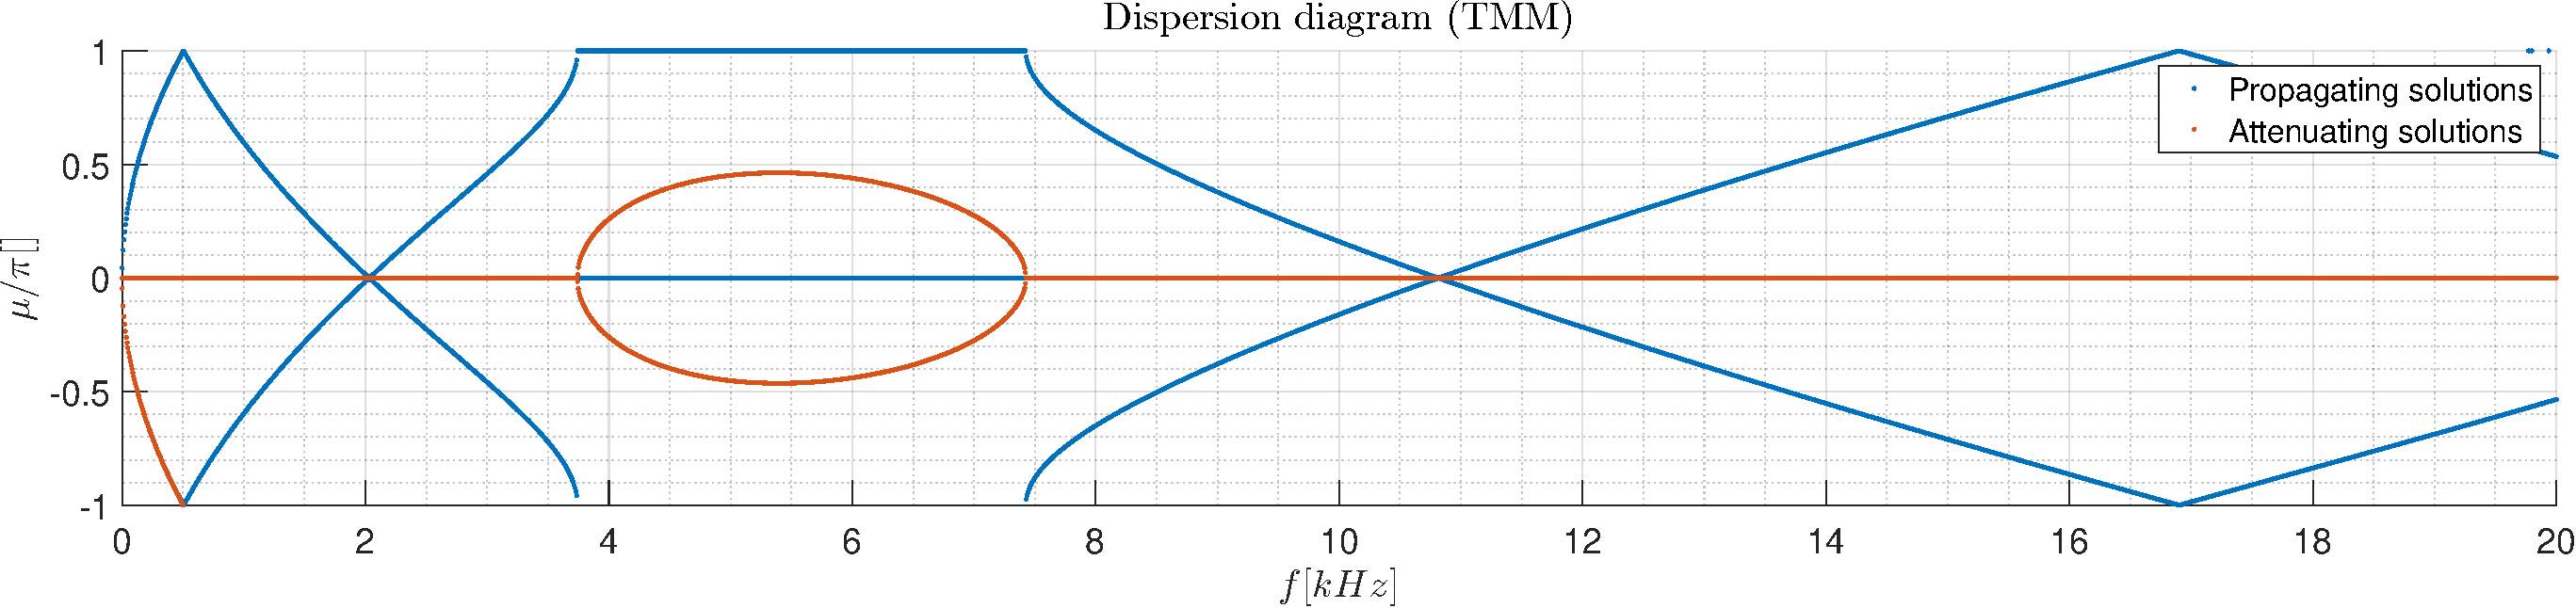
\includegraphics[width=\textwidth]{./img/MATLAB/TMM_ON-ON-ON_RLC_R0_L0_CInf.pdf}
            \caption{RLC shunt circuit with $R = 0 \Omega$, $L = 0 H$, and $C = \infty F$.}
        \end{figure}

    }

    \only<2-3>{

        \begin{figure}[H]
            \centering
            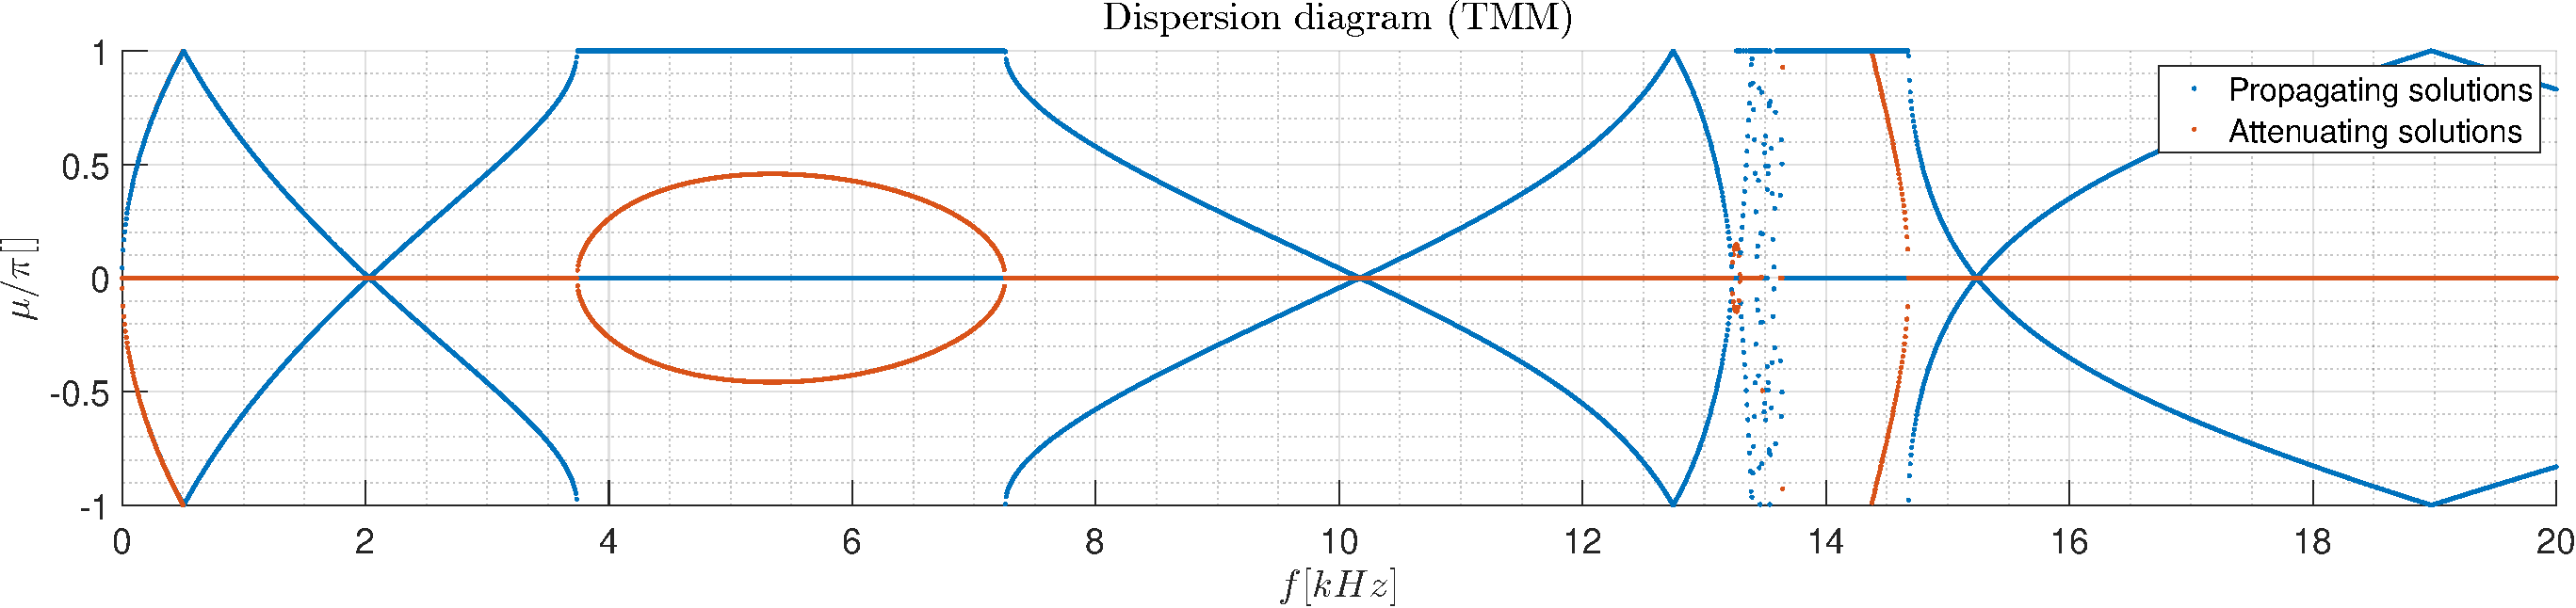
\includegraphics[width=\textwidth]{./img/MATLAB/TMM_ON-ON-ON_RLC_R0_L0.02_CInf.pdf}
            \caption{RLC shunt circuit with $R = 0 \Omega$, $L = 0.02 H$, and $C = \infty F$.}
        \end{figure}

    }

    \only<3-4>{

        \begin{figure}[H]
            \centering
            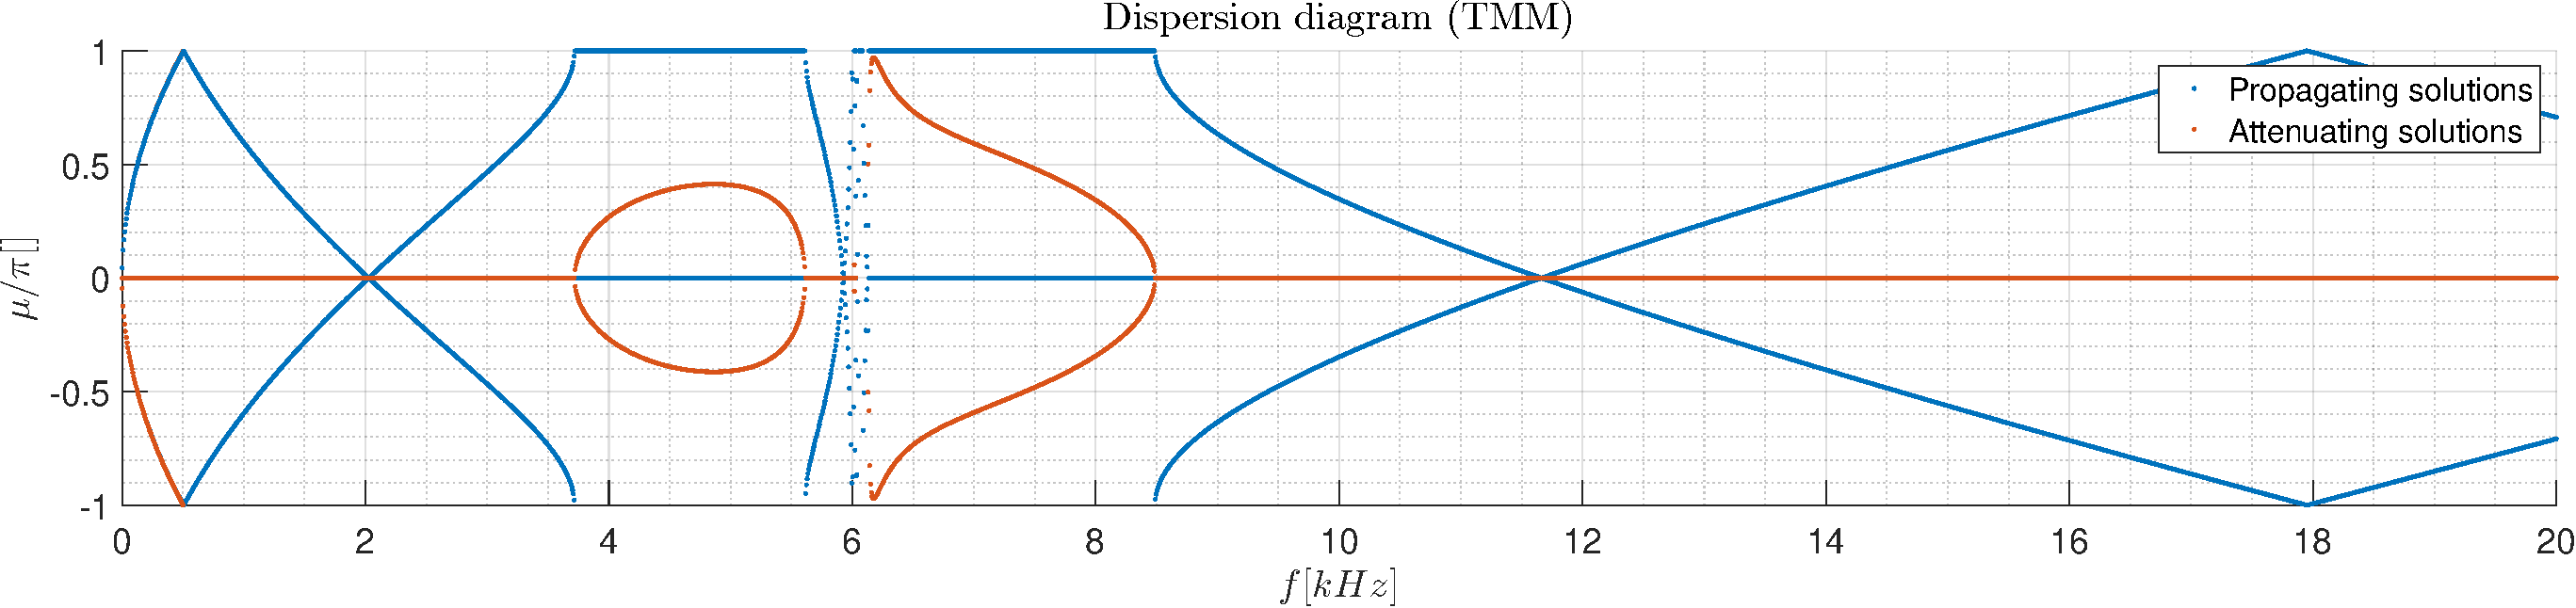
\includegraphics[width=\textwidth]{./img/MATLAB/TMM_ON-ON-ON_RLC_R0_L0.1_CInf.pdf}
            \caption{RLC shunt circuit with $R = 0 \Omega$, $L = 0.10 H$, and $C = \infty F$.}
        \end{figure}

    }

    \only<4->{

        \begin{figure}[H]
            \centering
            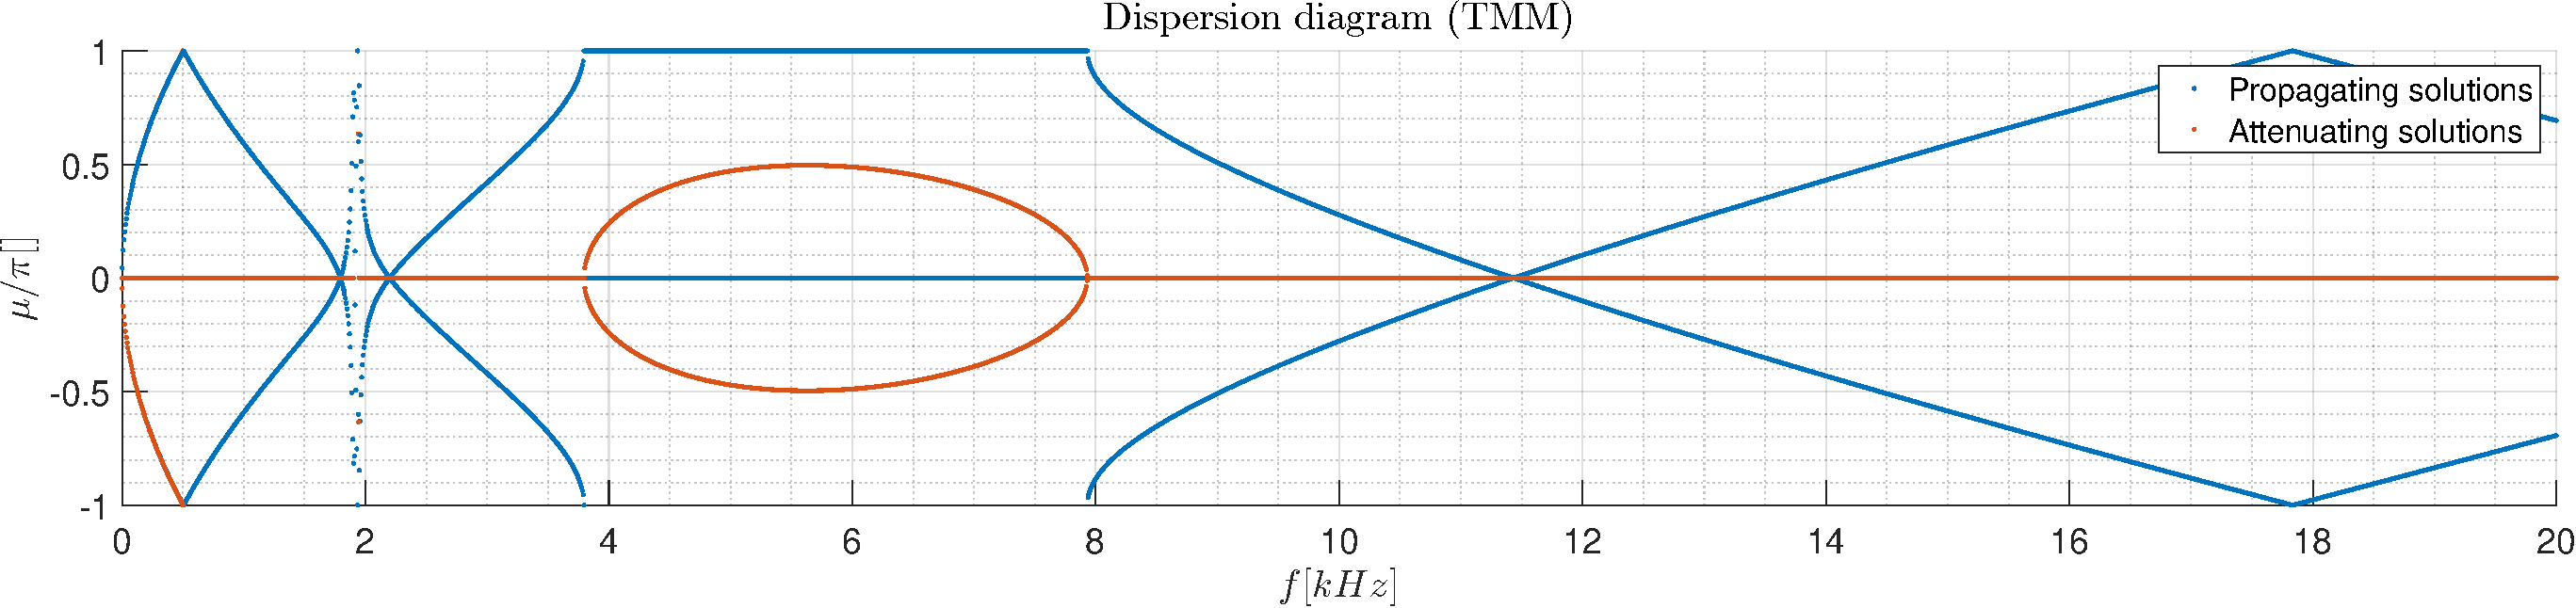
\includegraphics[width=\textwidth]{./img/MATLAB/TMM_ON-ON-ON_RLC_R0_L1_CInf.pdf}
            \caption{RLC shunt circuit with $R = 0 \Omega$, $L = 1 H$, and $C = \infty F$.}
        \end{figure}

    }

\end{frame}



\begin{frame}{$RL$ shunt circuit}

    \begin{figure}[H]
        \centering
        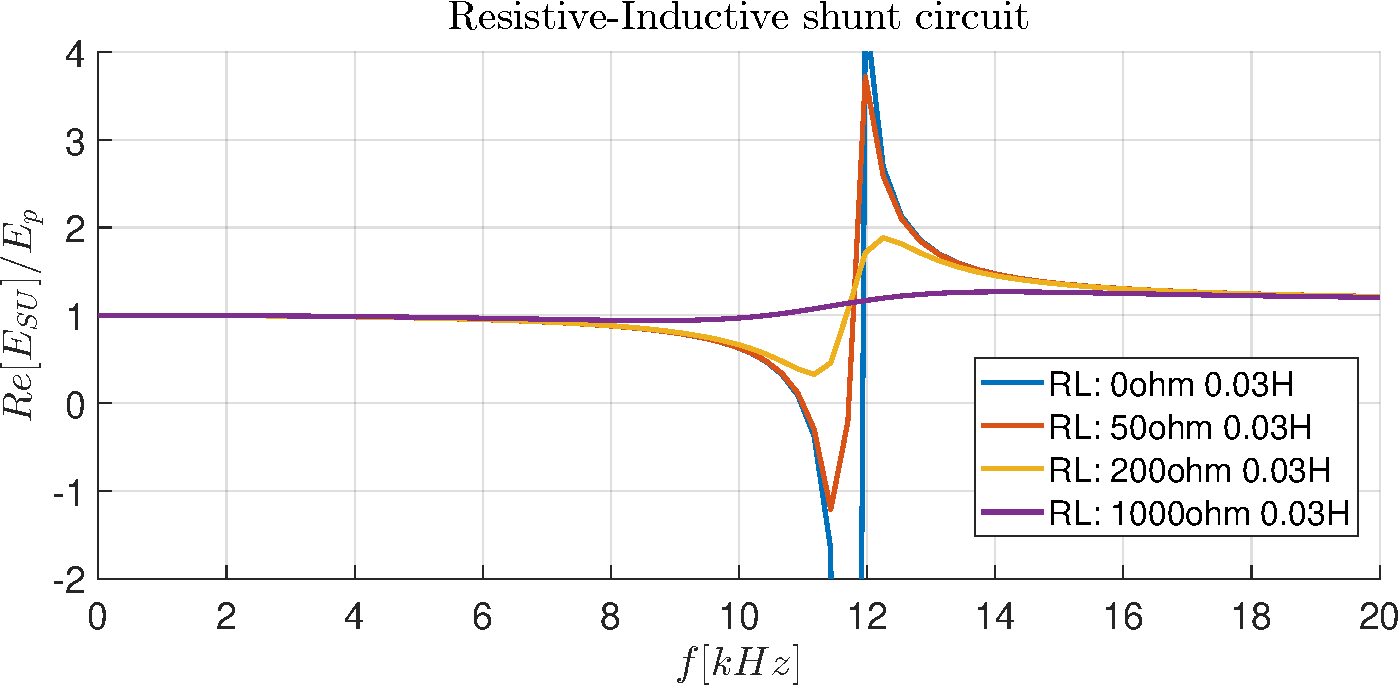
\includegraphics[width=0.6\textwidth]{./img/MATLAB/Y_SU_Resistive-Inductive shunt circuit.pdf}
        \caption{Analysis of $Y^{SU}$ for the resistive-inductive shunt circuit.}
    \end{figure}

    In case of $RL$ shunt circuit, mechanical admittance of the piezoelectric patches is given by:

    \begin{equation}
        Y^{SU} = Y_1^D \left( 1 - \frac{k_{31}^2}{1 -\omega^2 C_p^S L - s C_p^S R} \right)
    \end{equation}

    The resistive element $R$ acts as a damping factor, controlling the width and depth of the band-gap.
    For high values of $R$, the band-gap can be completely suppressed.

\end{frame}


\begin{frame}{$RL$ shunt circuit}


    \only<1-2>{

        \begin{figure}[H]
            \centering
            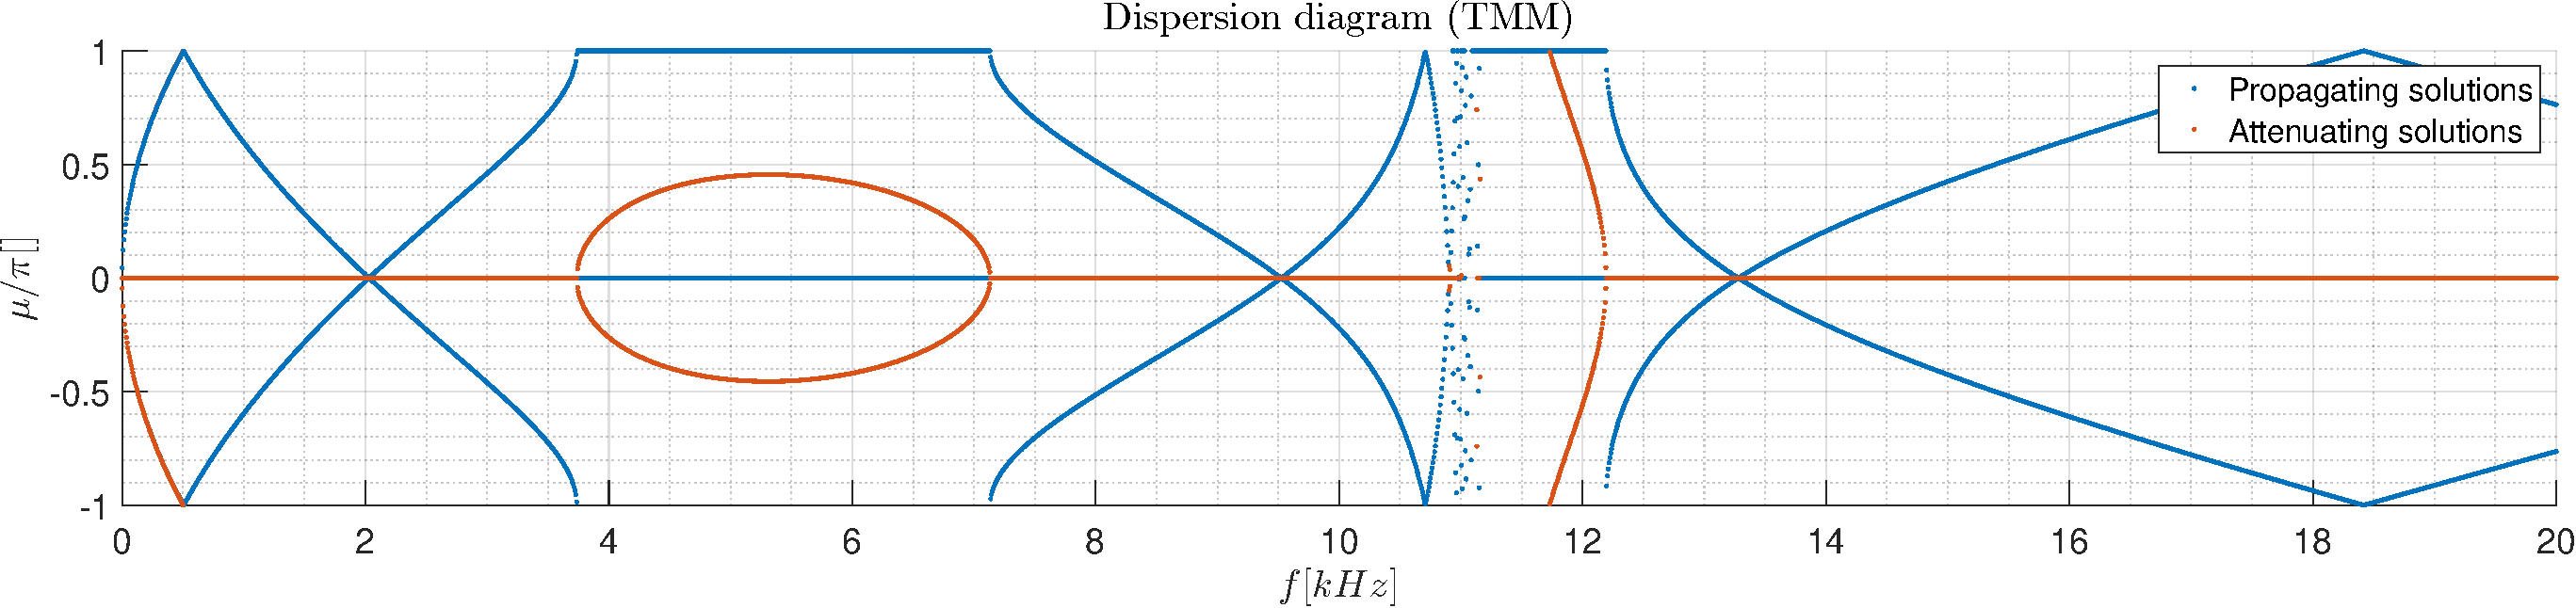
\includegraphics[width=\textwidth]{./img/MATLAB/TMM_ON-ON-ON_RLC_R0_L0.03_CInf.pdf}
            \caption{RLC shunt circuit with $R = 0 \Omega$, $L = 0.03 H$, and $C = \infty F$.}

        \end{figure}

    }

    \only<2-3>{

        \begin{figure}[H]
            \centering
            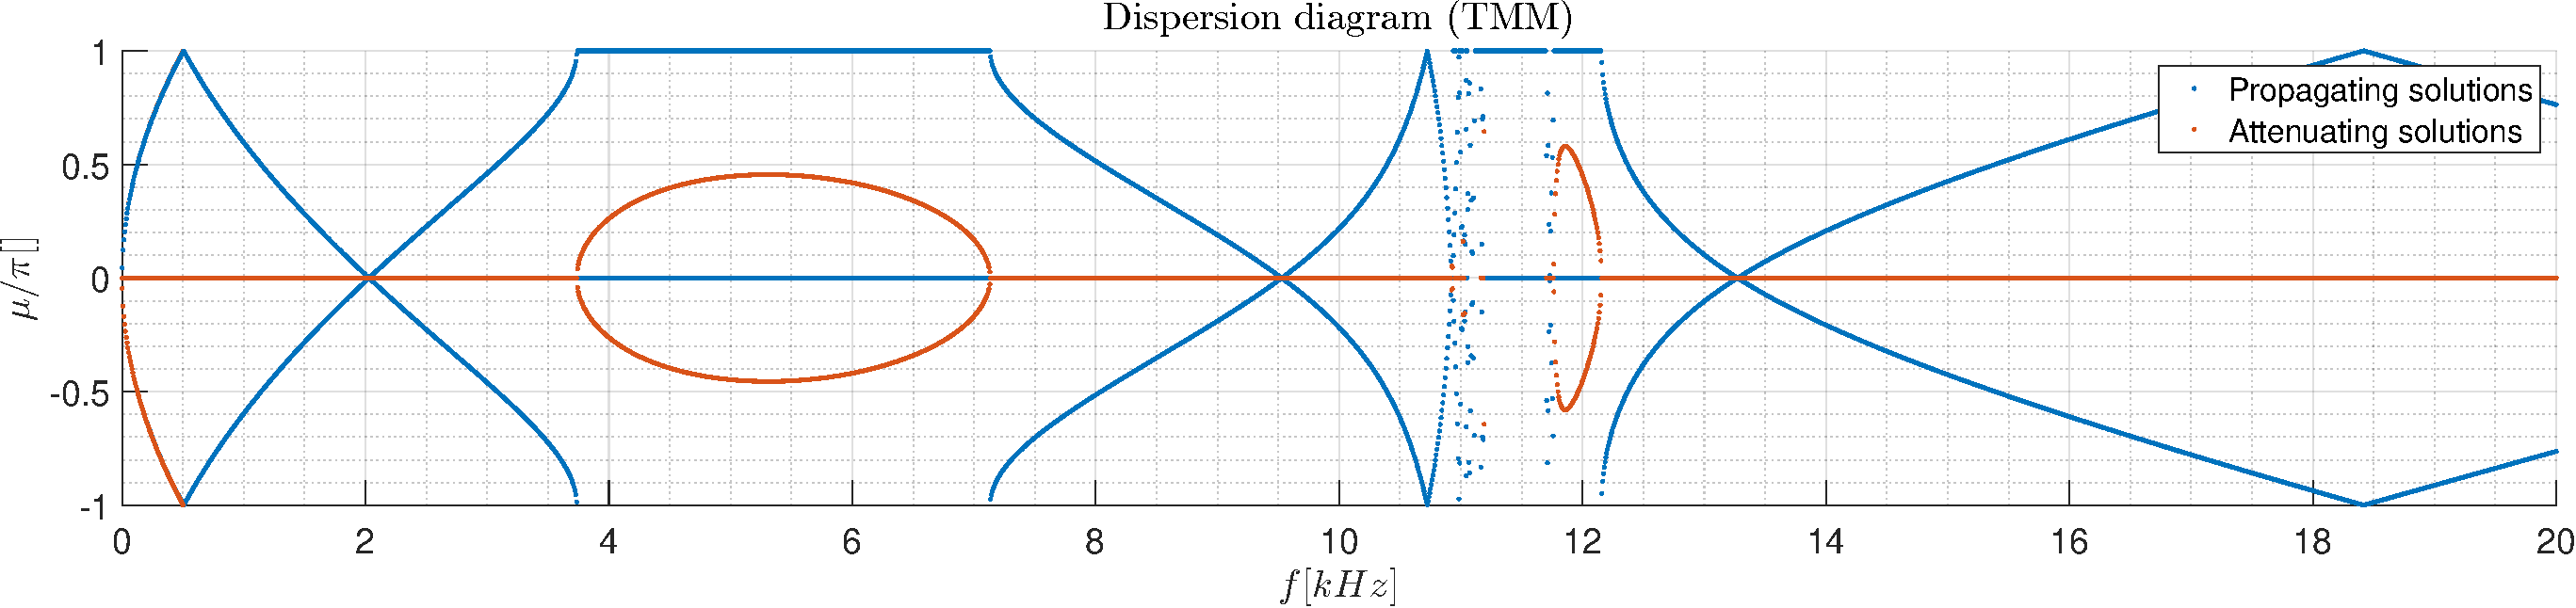
\includegraphics[width=\textwidth]{./img/MATLAB/TMM_ON-ON-ON_RLC_R50_L0.03_CInf.pdf}
            \caption{RLC shunt circuit with $R = 50 \Omega$, $L = 0.03 H$, and $C = \infty F$.}

        \end{figure}

    }

    \only<3-4>{

        \begin{figure}[H]
            \centering
            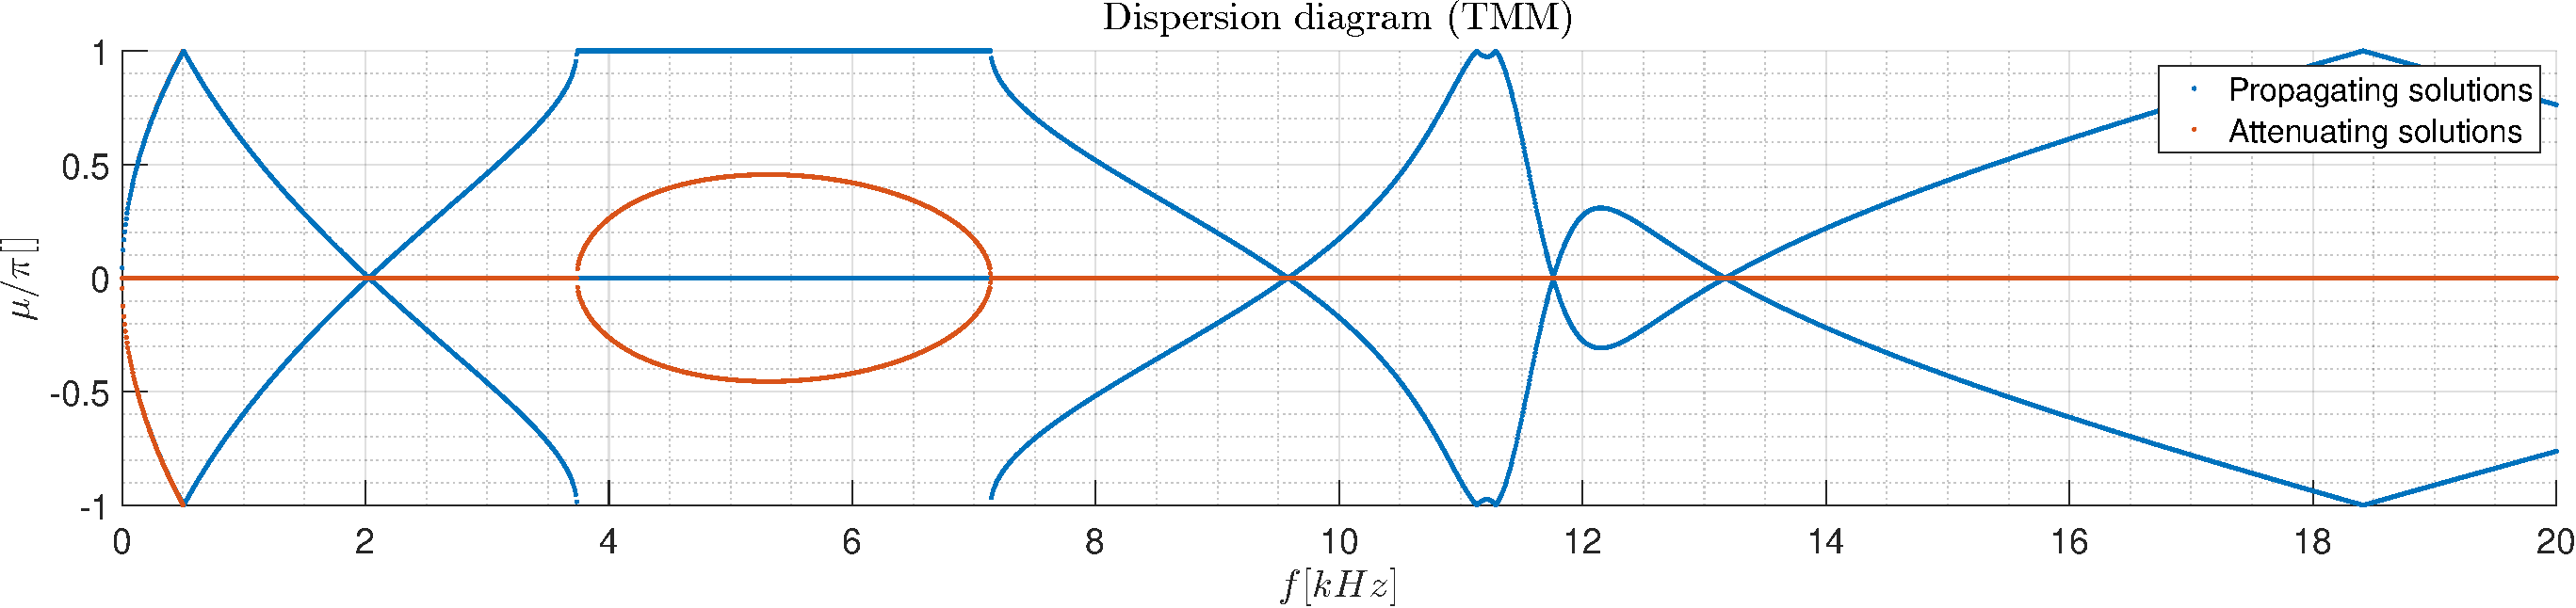
\includegraphics[width=\textwidth]{./img/MATLAB/TMM_ON-ON-ON_RLC_R200_L0.03_CInf.pdf}
            \caption{RLC shunt circuit with $R = 200 \Omega$, $L = 0.03 H$, and $C = \infty F$.}

        \end{figure}

    }

    \only<4->{

        \begin{figure}[H]
            \centering
            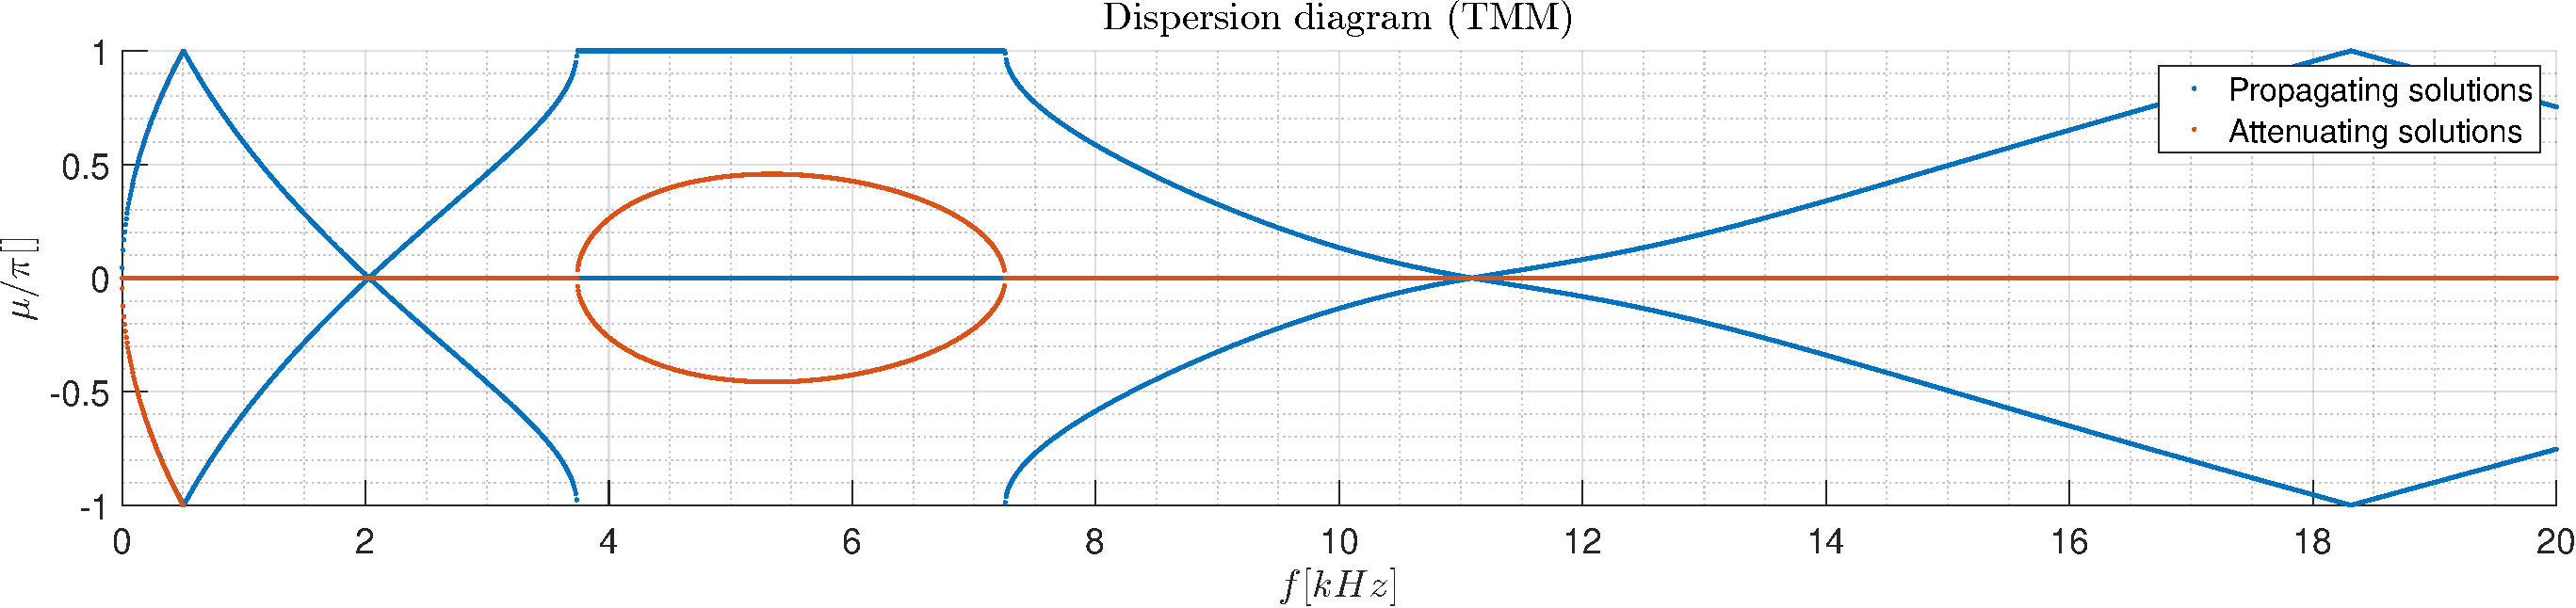
\includegraphics[width=\textwidth]{./img/MATLAB/TMM_ON-ON-ON_RLC_R1000_L0.03_CInf.pdf}
            \caption{RLC shunt circuit with $R = 1000 \Omega$, $L = 0.03 H$, and $C = \infty F$.}
        \end{figure}

    }

\end{frame}



\begin{frame}{$RC_N$ shunt circuit}

    \begin{figure}[H]
        \centering
        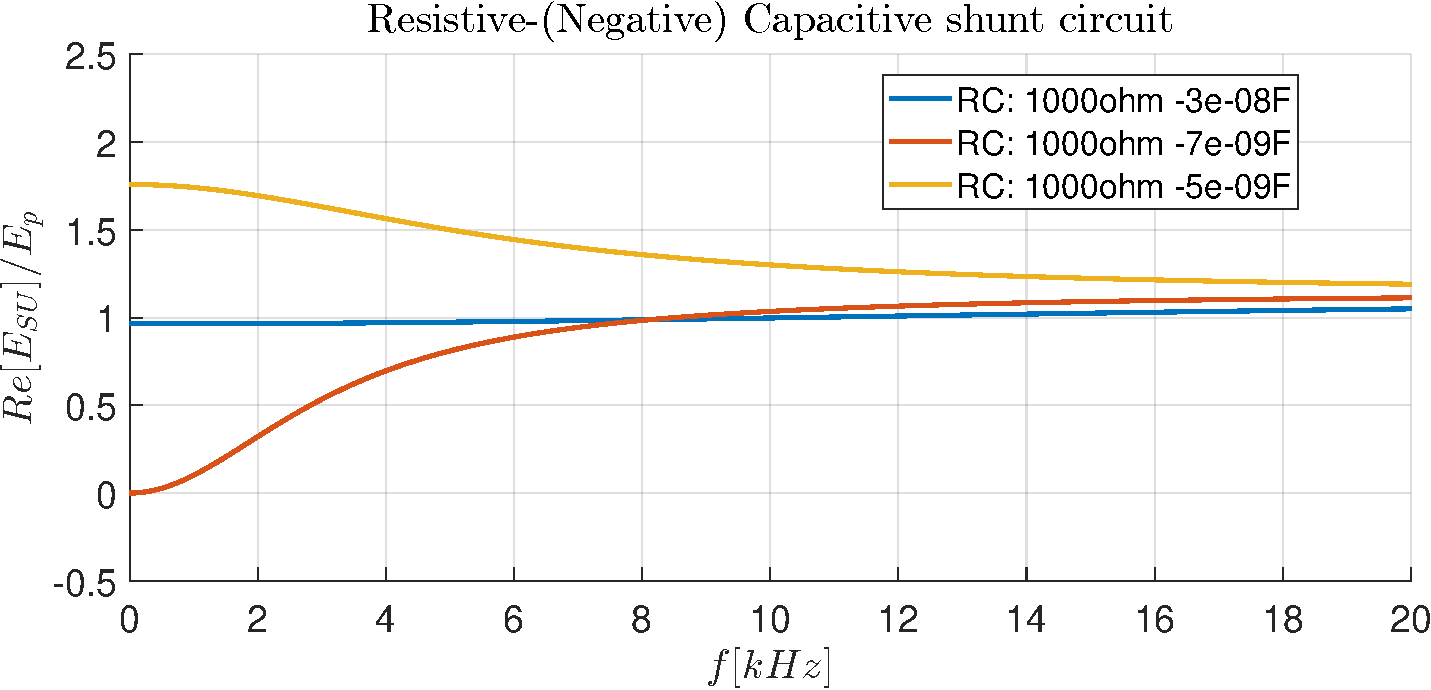
\includegraphics[width=0.6\textwidth]{./img/MATLAB/Y_SU_Resistive-(Negative) Capacitive shunt circuit.pdf}
        \caption{Analysis of $Y^{SU}$ for the resistive-(negative) capacitive shunt circuit.}
    \end{figure}

    In case of $RC_N$ shunt circuit, mechanical admittance of the piezoelectric patches is given by:

    \begin{equation}
        Y^{SU} = Y_1^D \left( 1 - \frac{k_{31}^2}{1 - C_p^S \frac{1}{C_N} - s C_p^S R} \right)
    \end{equation}

    The capacitative element has similar effects as the inductive one, with the ability to shift the band-gap toward lower or higher frequencies depending on the sign of $1 - C_p^S \frac{1}{C_N}$.

\end{frame}



\begin{frame}{$RC_N$ shunt circuit}

    \only<1-2>{

        \begin{figure}[H]
            \centering
            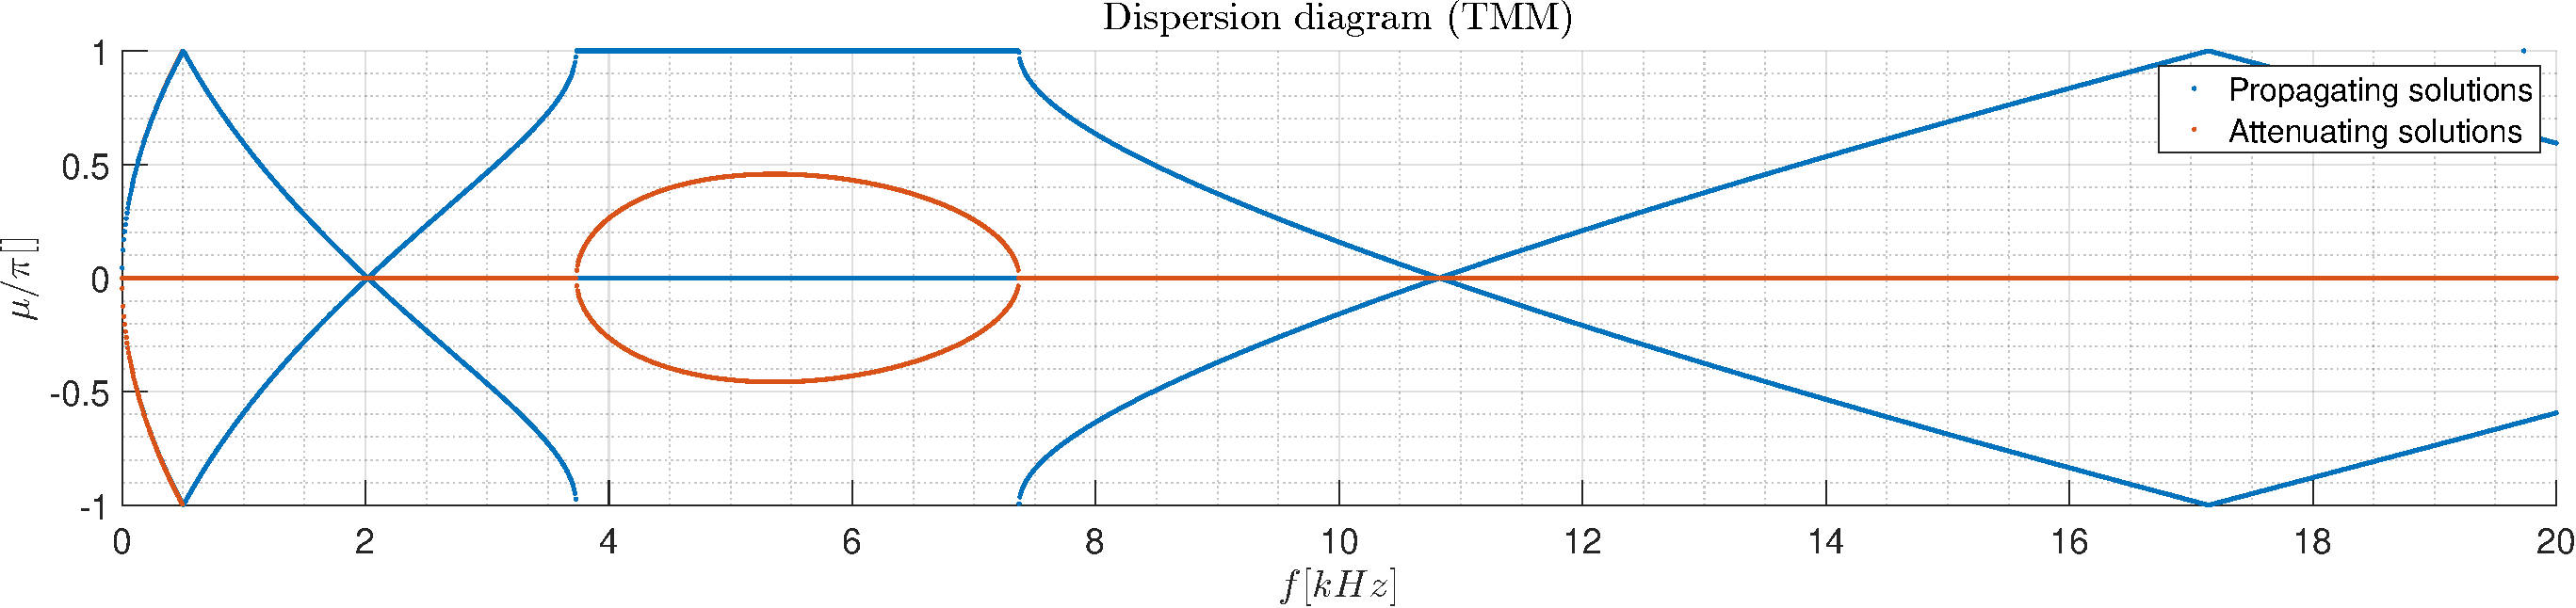
\includegraphics[width=\textwidth]{./img/MATLAB/TMM_ON-ON-ON_RLC_R1000_L0_C-3e-08.pdf}
            \caption{RLC shunt circuit with $R = 1000 \Omega$, $L = 0 H$, and $C = -30 nF$.}
        \end{figure}

    }

    \only<2-3>{

        \begin{figure}[H]
            \centering
            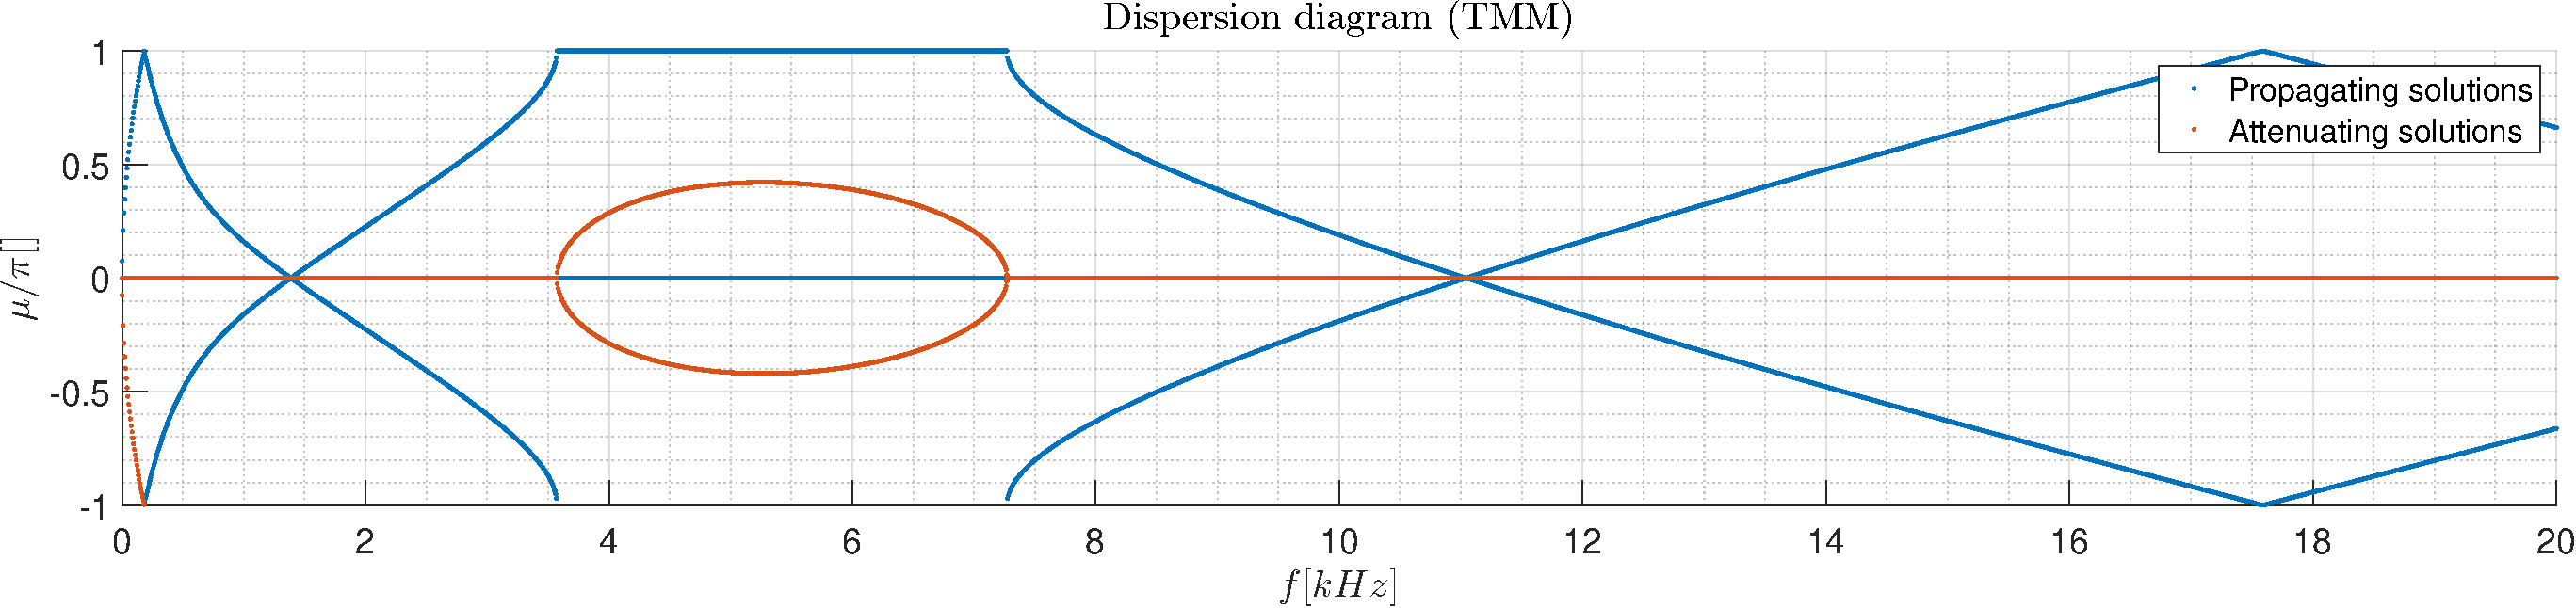
\includegraphics[width=\textwidth]{./img/MATLAB/TMM_ON-ON-ON_RLC_R1000_L0_C-7e-09.pdf}
            \caption{RLC shunt circuit with $R = 1000 \Omega$, $L = 0 H$, and $C = -7 nF$.}
        \end{figure}

    }

    \only<3->{

        \begin{figure}[H]
            \centering
            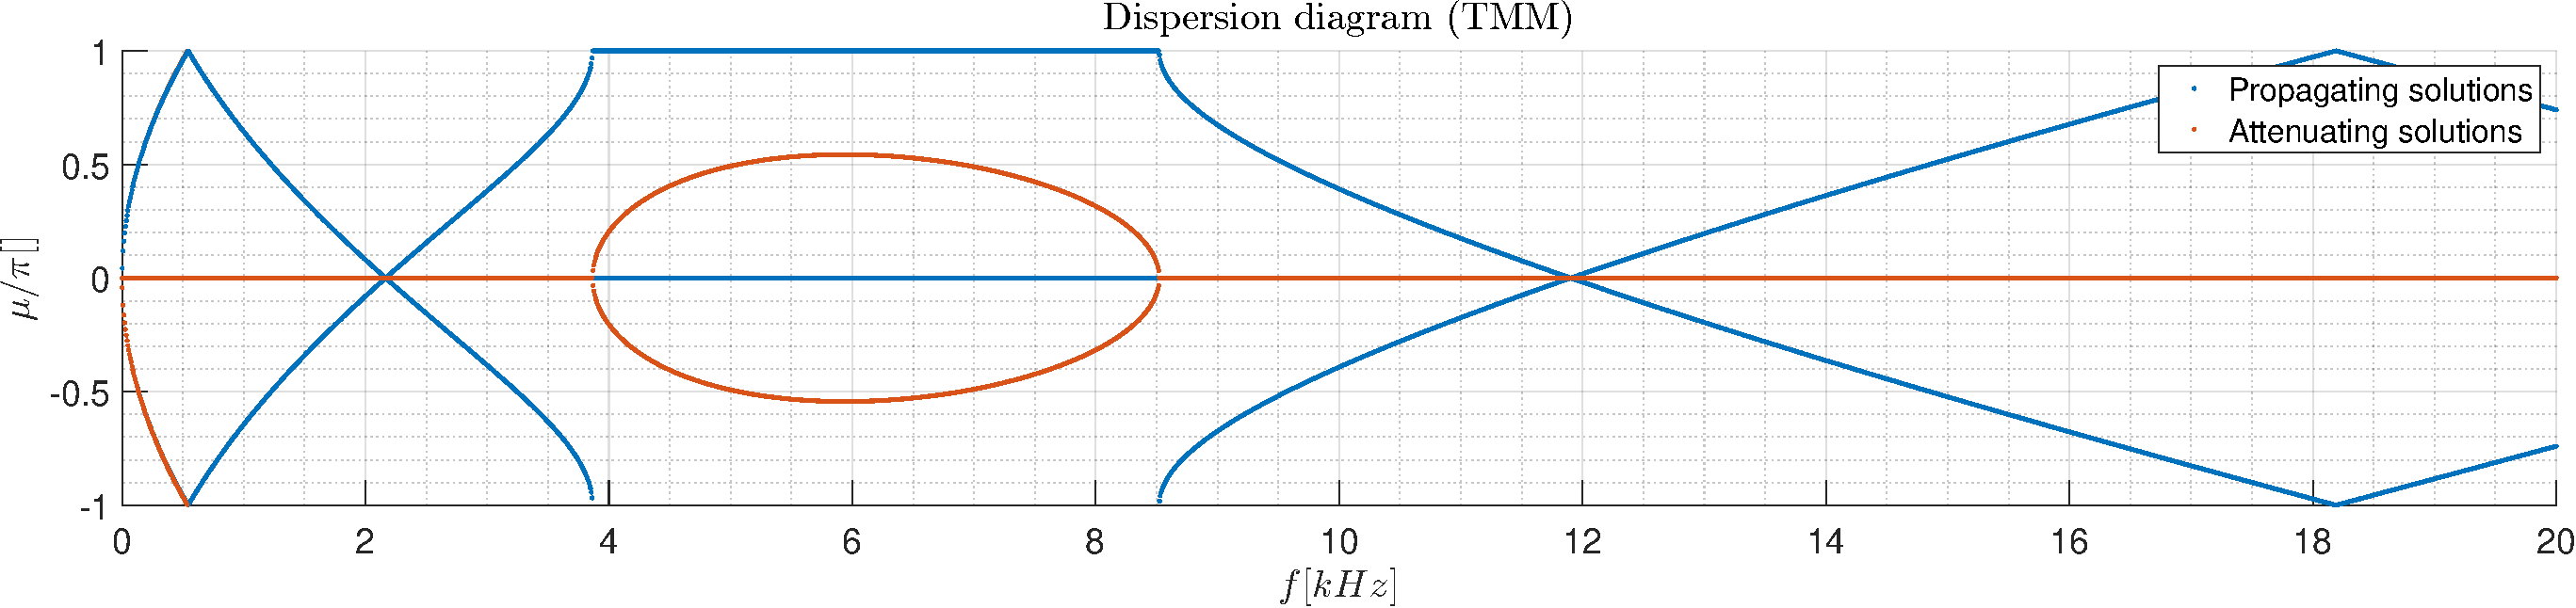
\includegraphics[width=\textwidth]{./img/MATLAB/TMM_ON-ON-ON_RLC_R1000_L0_C-5e-09.pdf}
            \caption{RLC shunt circuit with $R = 1000 \Omega$, $L = 0 H$, and $C = -5 nF$.}
        \end{figure}

    }

\end{frame}

\section{Experimental results}


\subsection{Space-Only modulation}

\begin{frame}{Space-Only modulation}

    \begin{columns}[c, onlytextwidth]

        \begin{column}{0.55\textwidth}

            In the case of space-only modulation, piezoelectric patches can be either in the short-circuit (ON) or open-circuit (OFF) state.
            Three different configurations of the ST cell are considered:

            \begin{itemize}
                \item \textit{OFF-OFF-OFF}
                \item \textit{ON-ON-ON}
                \item \textit{ON-OFF-OFF}
            \end{itemize}

        \end{column}

        \begin{column}{0.45\textwidth}

            \begin{figure}[H]
                \centering
                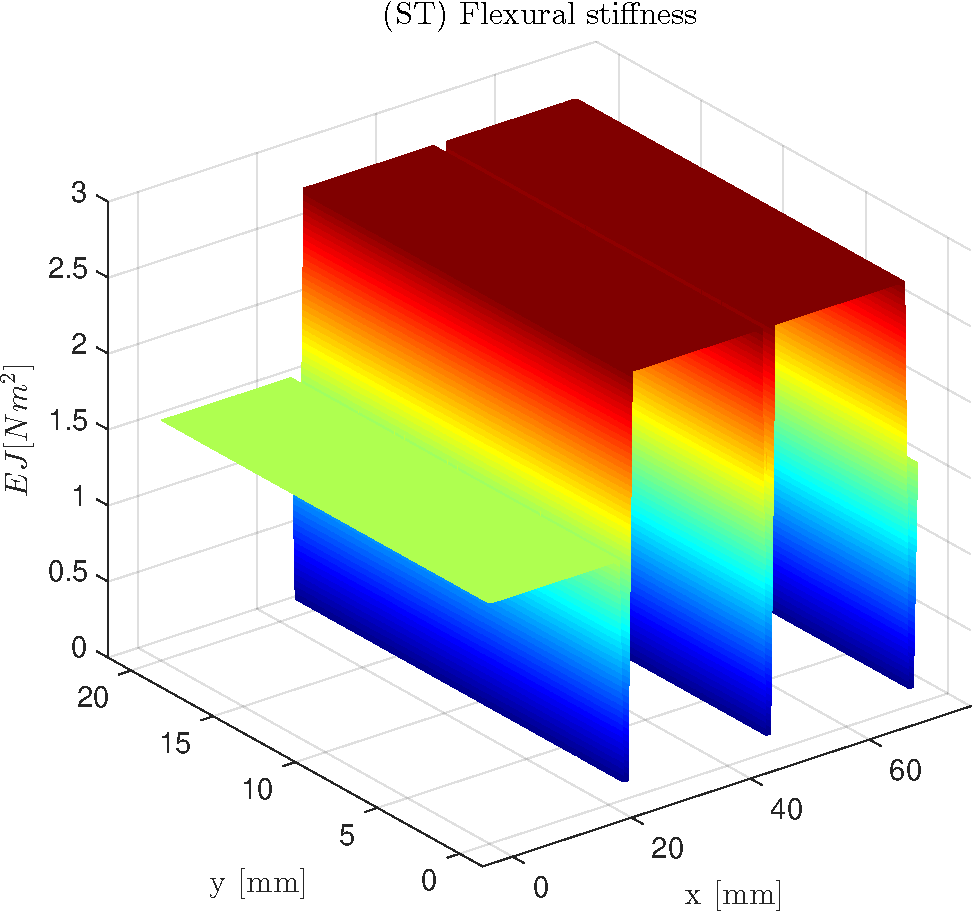
\includegraphics[width=0.9\textwidth]{img/MATLAB/ST_cell_ON-OFF-OFF.pdf}
                \caption{ST cell in the case \textit{ON-OFF-OFF}.}
            \end{figure}

        \end{column}

    \end{columns}

    \vspace{9pt}

    Numerical simulations performed using TMM\footnotemark[1] and PWEM\footnotemark[2] are compared against experimental data.
    \texttt{Comsol Multiphysics} is also adopted as a valid reference.

    \footnotetext[1]{Transfer Matrix Method}
    \footnotetext[2]{Plane Wave Expansion Method}

\end{frame}



\begin{frame}{Case \textit{OFF-OFF-OFF}}

    The first band-gap is observed at $f_{BG}^{OFF-OFF-OFF} = [3.8, 7.5] kHz$.

    \begin{figure}[H]
        \centering
        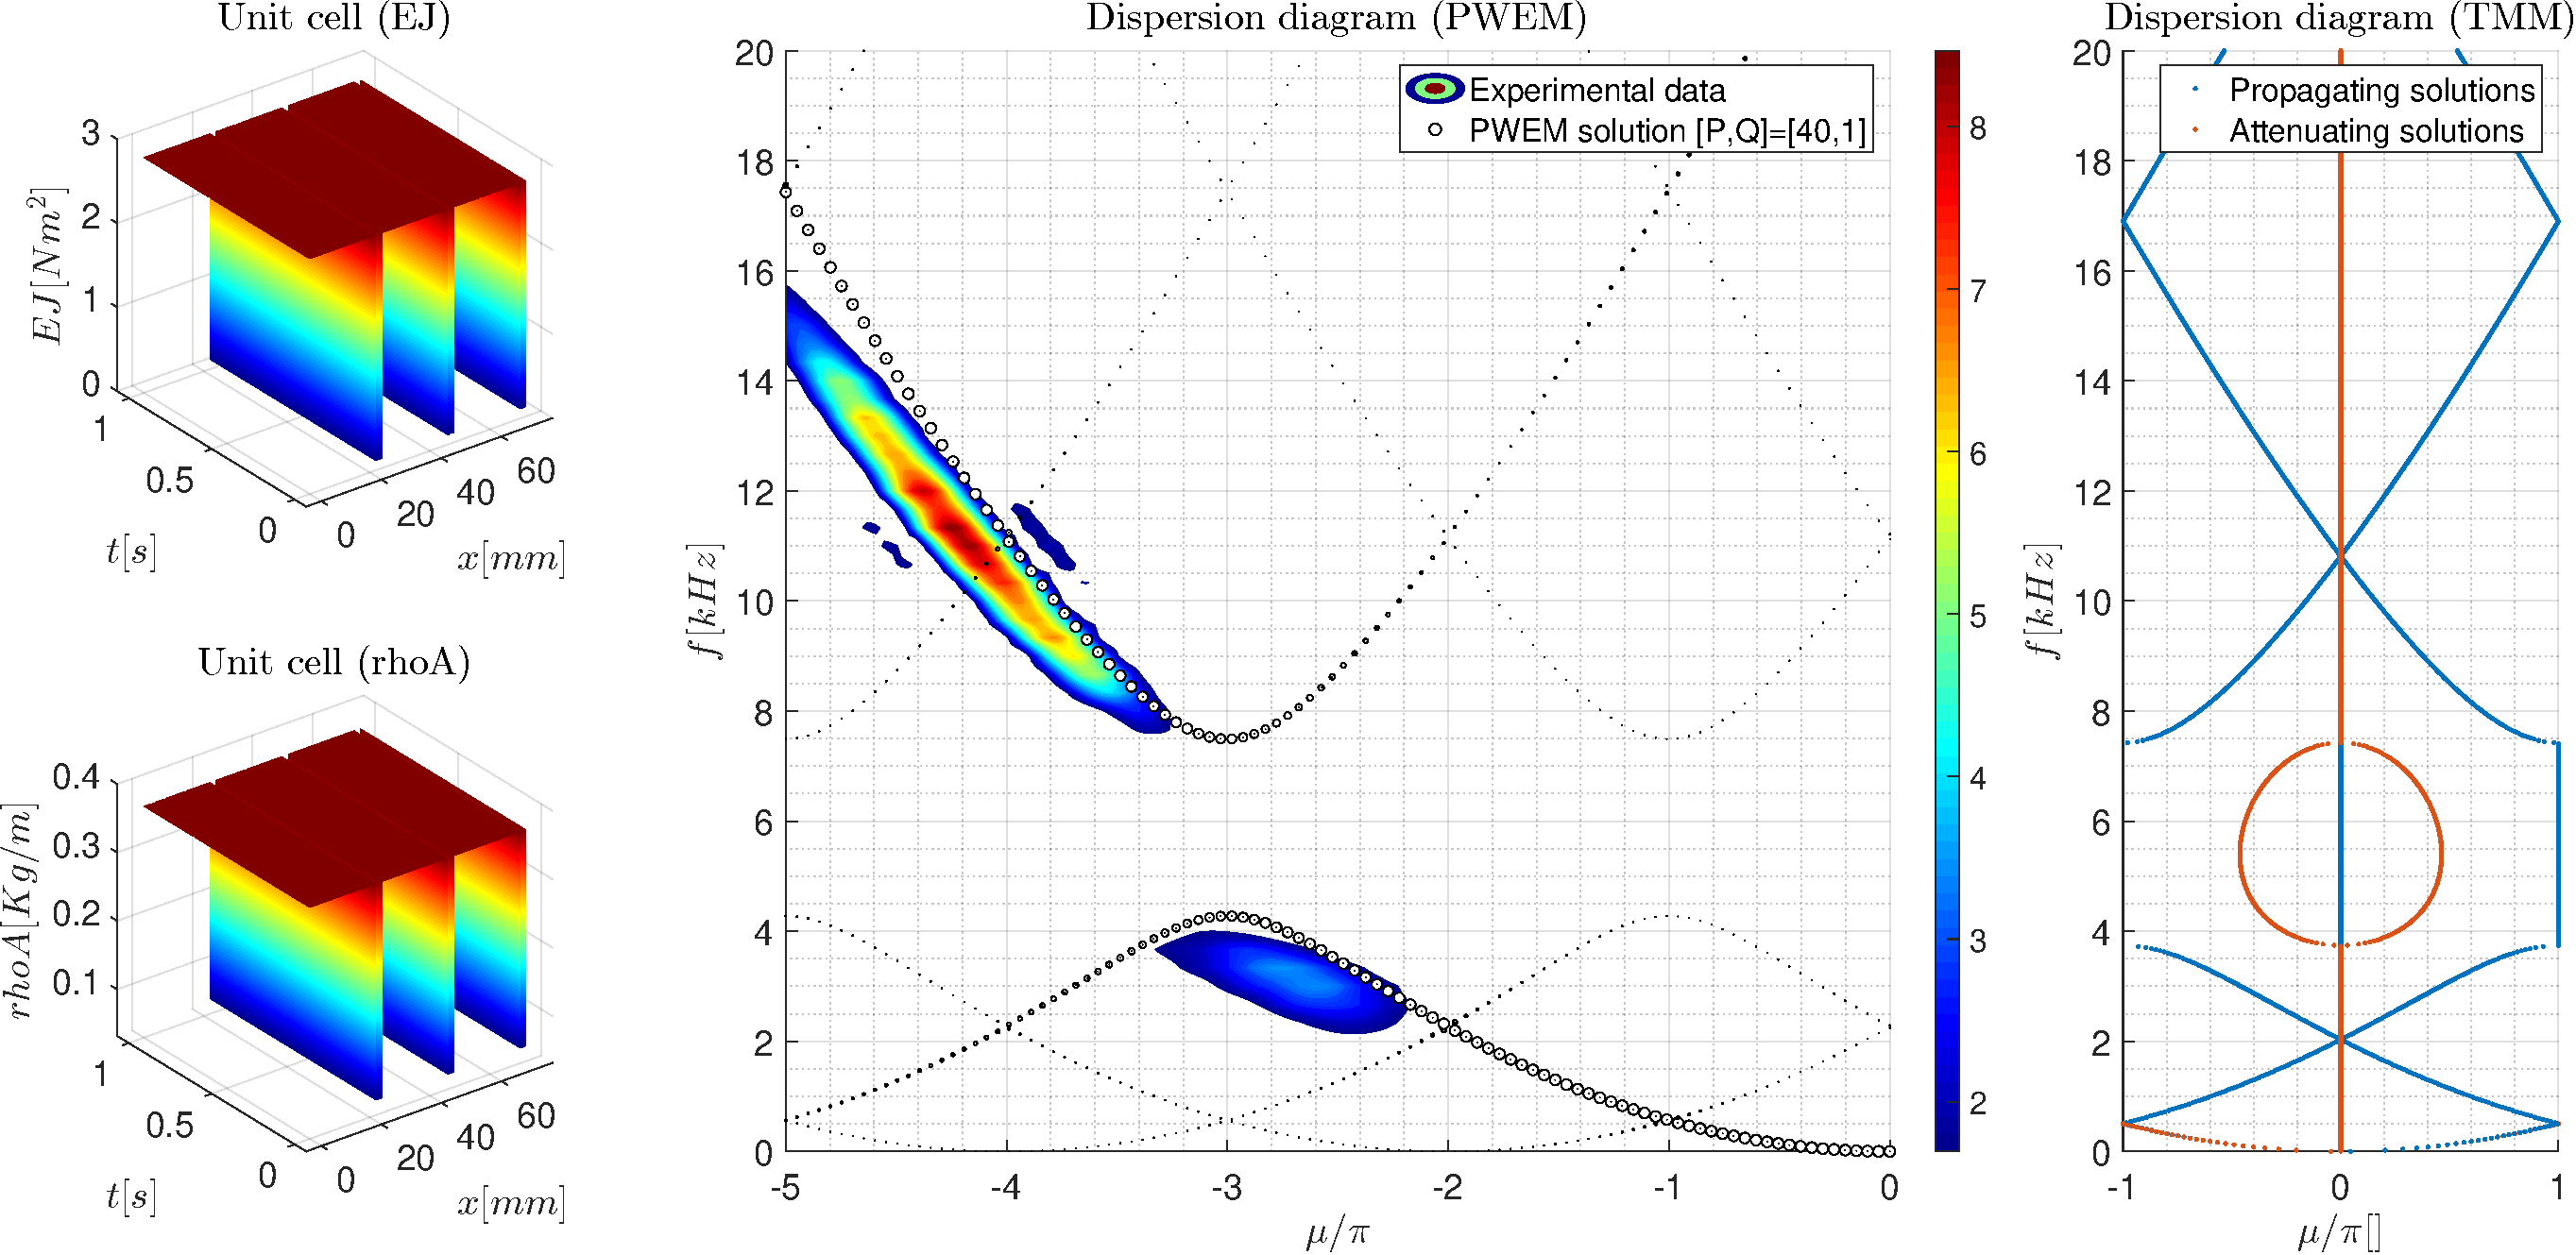
\includegraphics[width=\textwidth]{./img/MATLAB/PWEM_TMM_EXP OFF-OFF-OFF @0kHz.pdf}
        \caption{Dispersion diagram for the OFF-OFF-OFF configuration.}
    \end{figure}

\end{frame}



\begin{frame}{Case \textit{ON-ON-ON}}

    Short-circuiting all the piezoelectric patches results in a decrease of the structural stiffness and a shift of the band-gap towards lower frequencies ($f_{BG}^{ON-ON-ON} = [3.4, 5.6] kHz$).

    \begin{figure}[H]
        \centering
        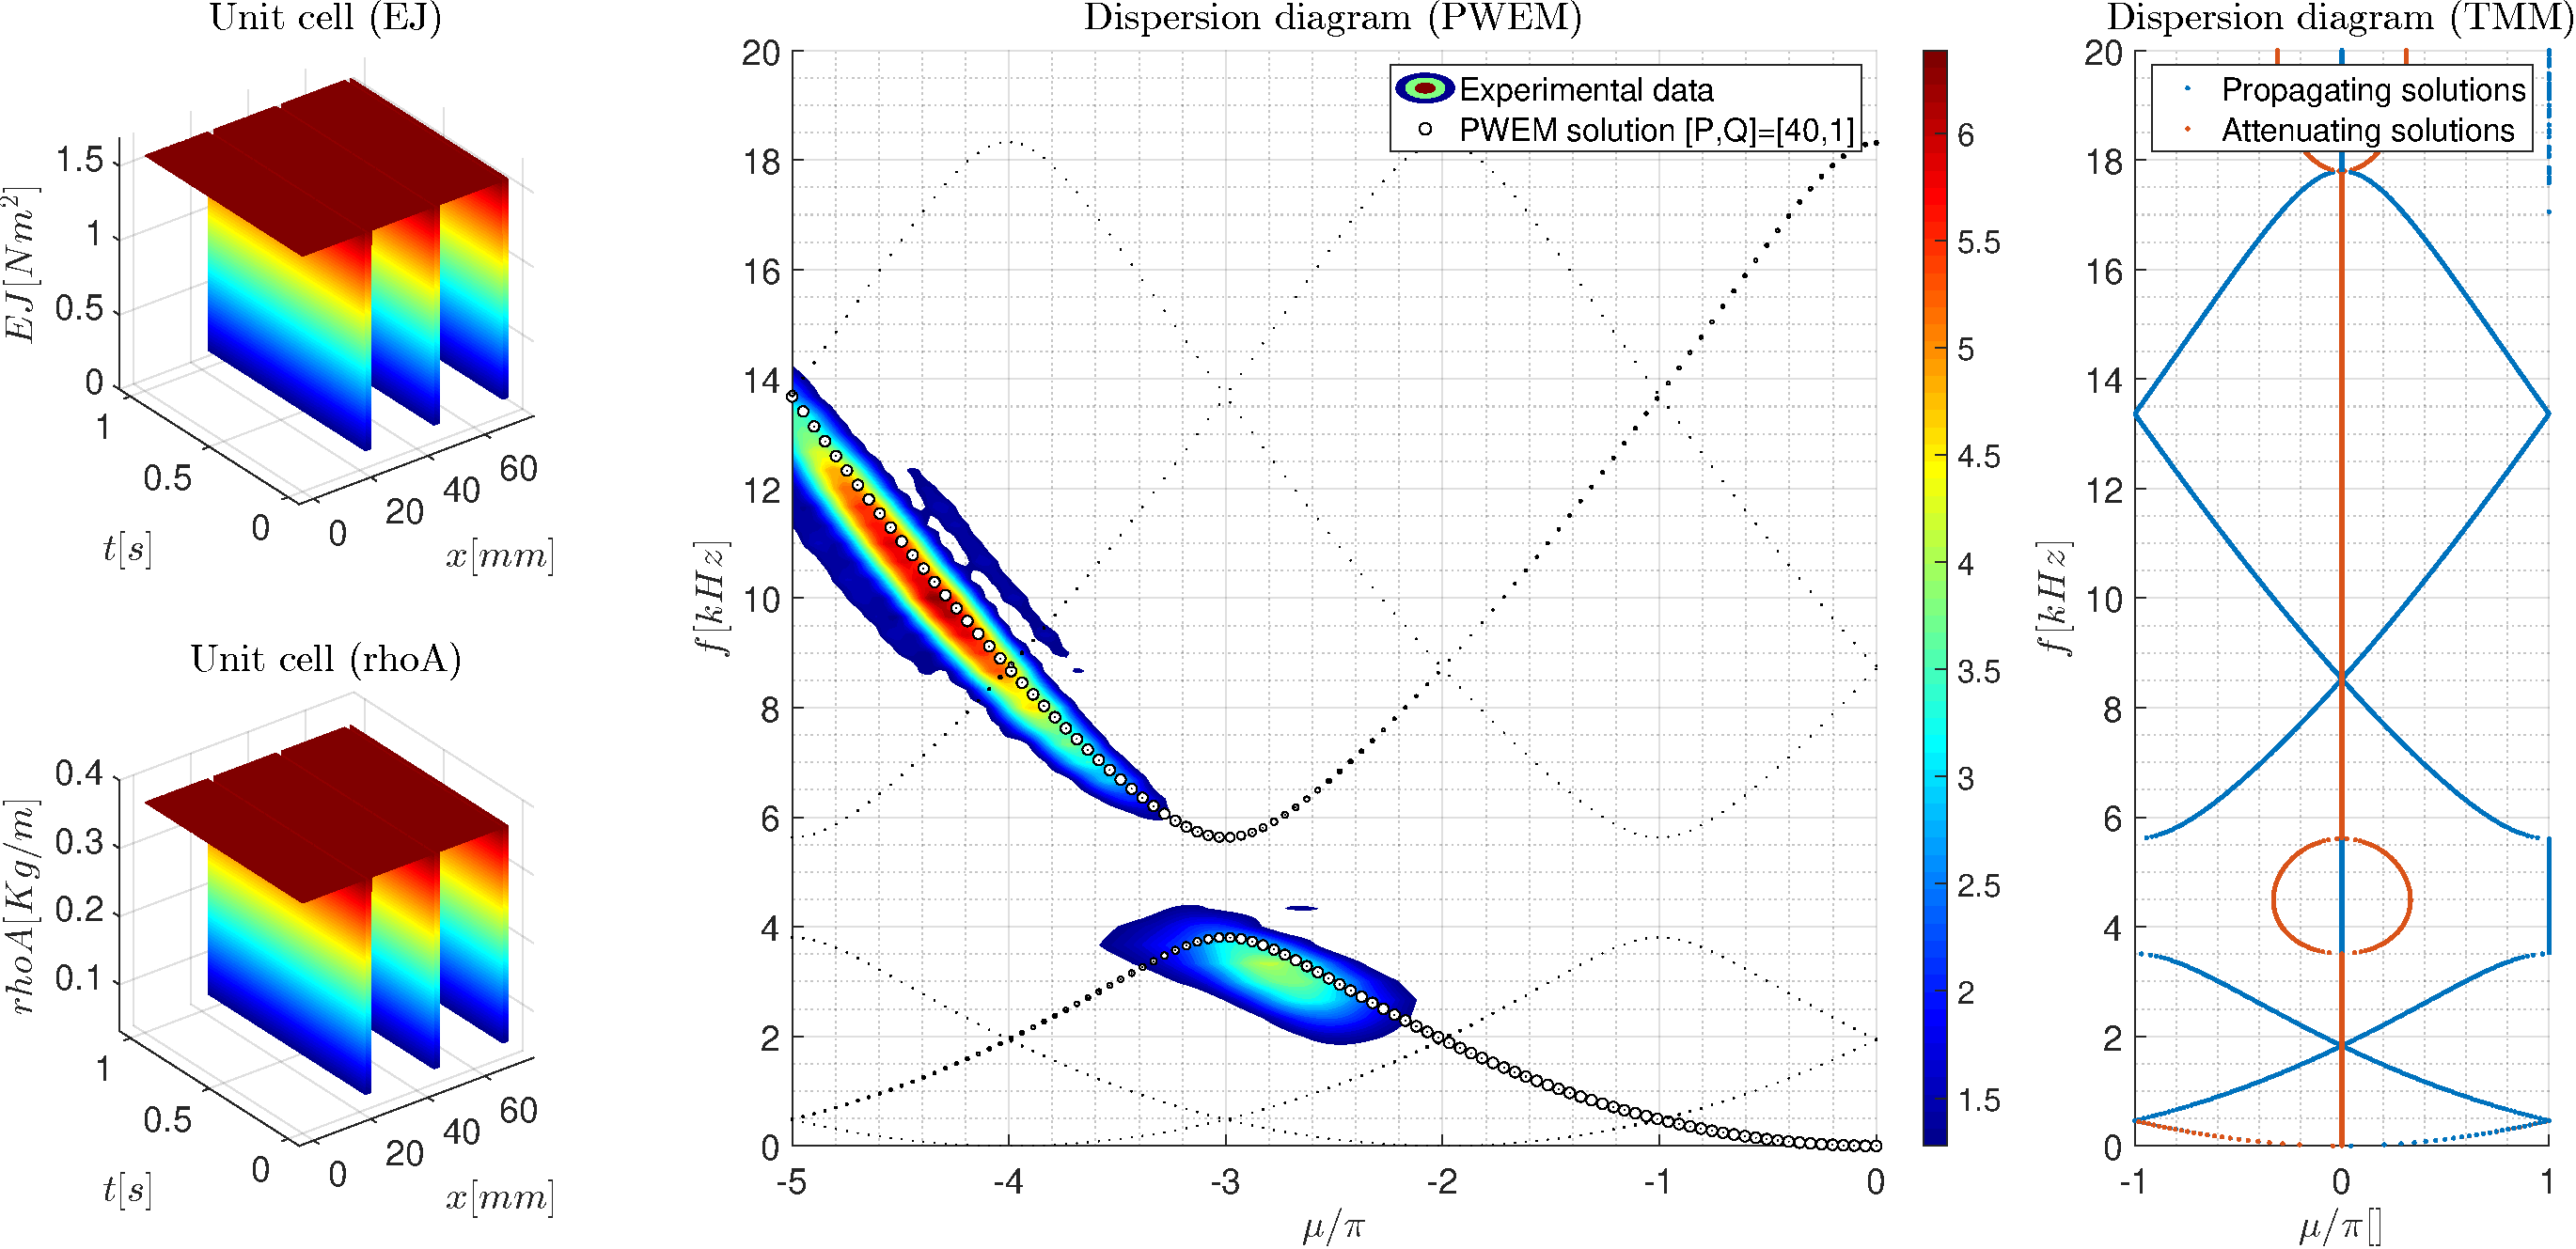
\includegraphics[width=\textwidth]{./img/MATLAB/PWEM_TMM_EXP ON-ON-ON @0kHz.pdf}
        \caption{Dispersion diagram for the ON-ON-ON configuration.}
    \end{figure}

\end{frame}



\begin{frame}{Case \textit{ON-OFF-OFF}}

    The introduction of additional sources of dispersion in the system results in a higher number of band-gaps visible in the same frequency range.

    \begin{figure}[H]
        \centering
        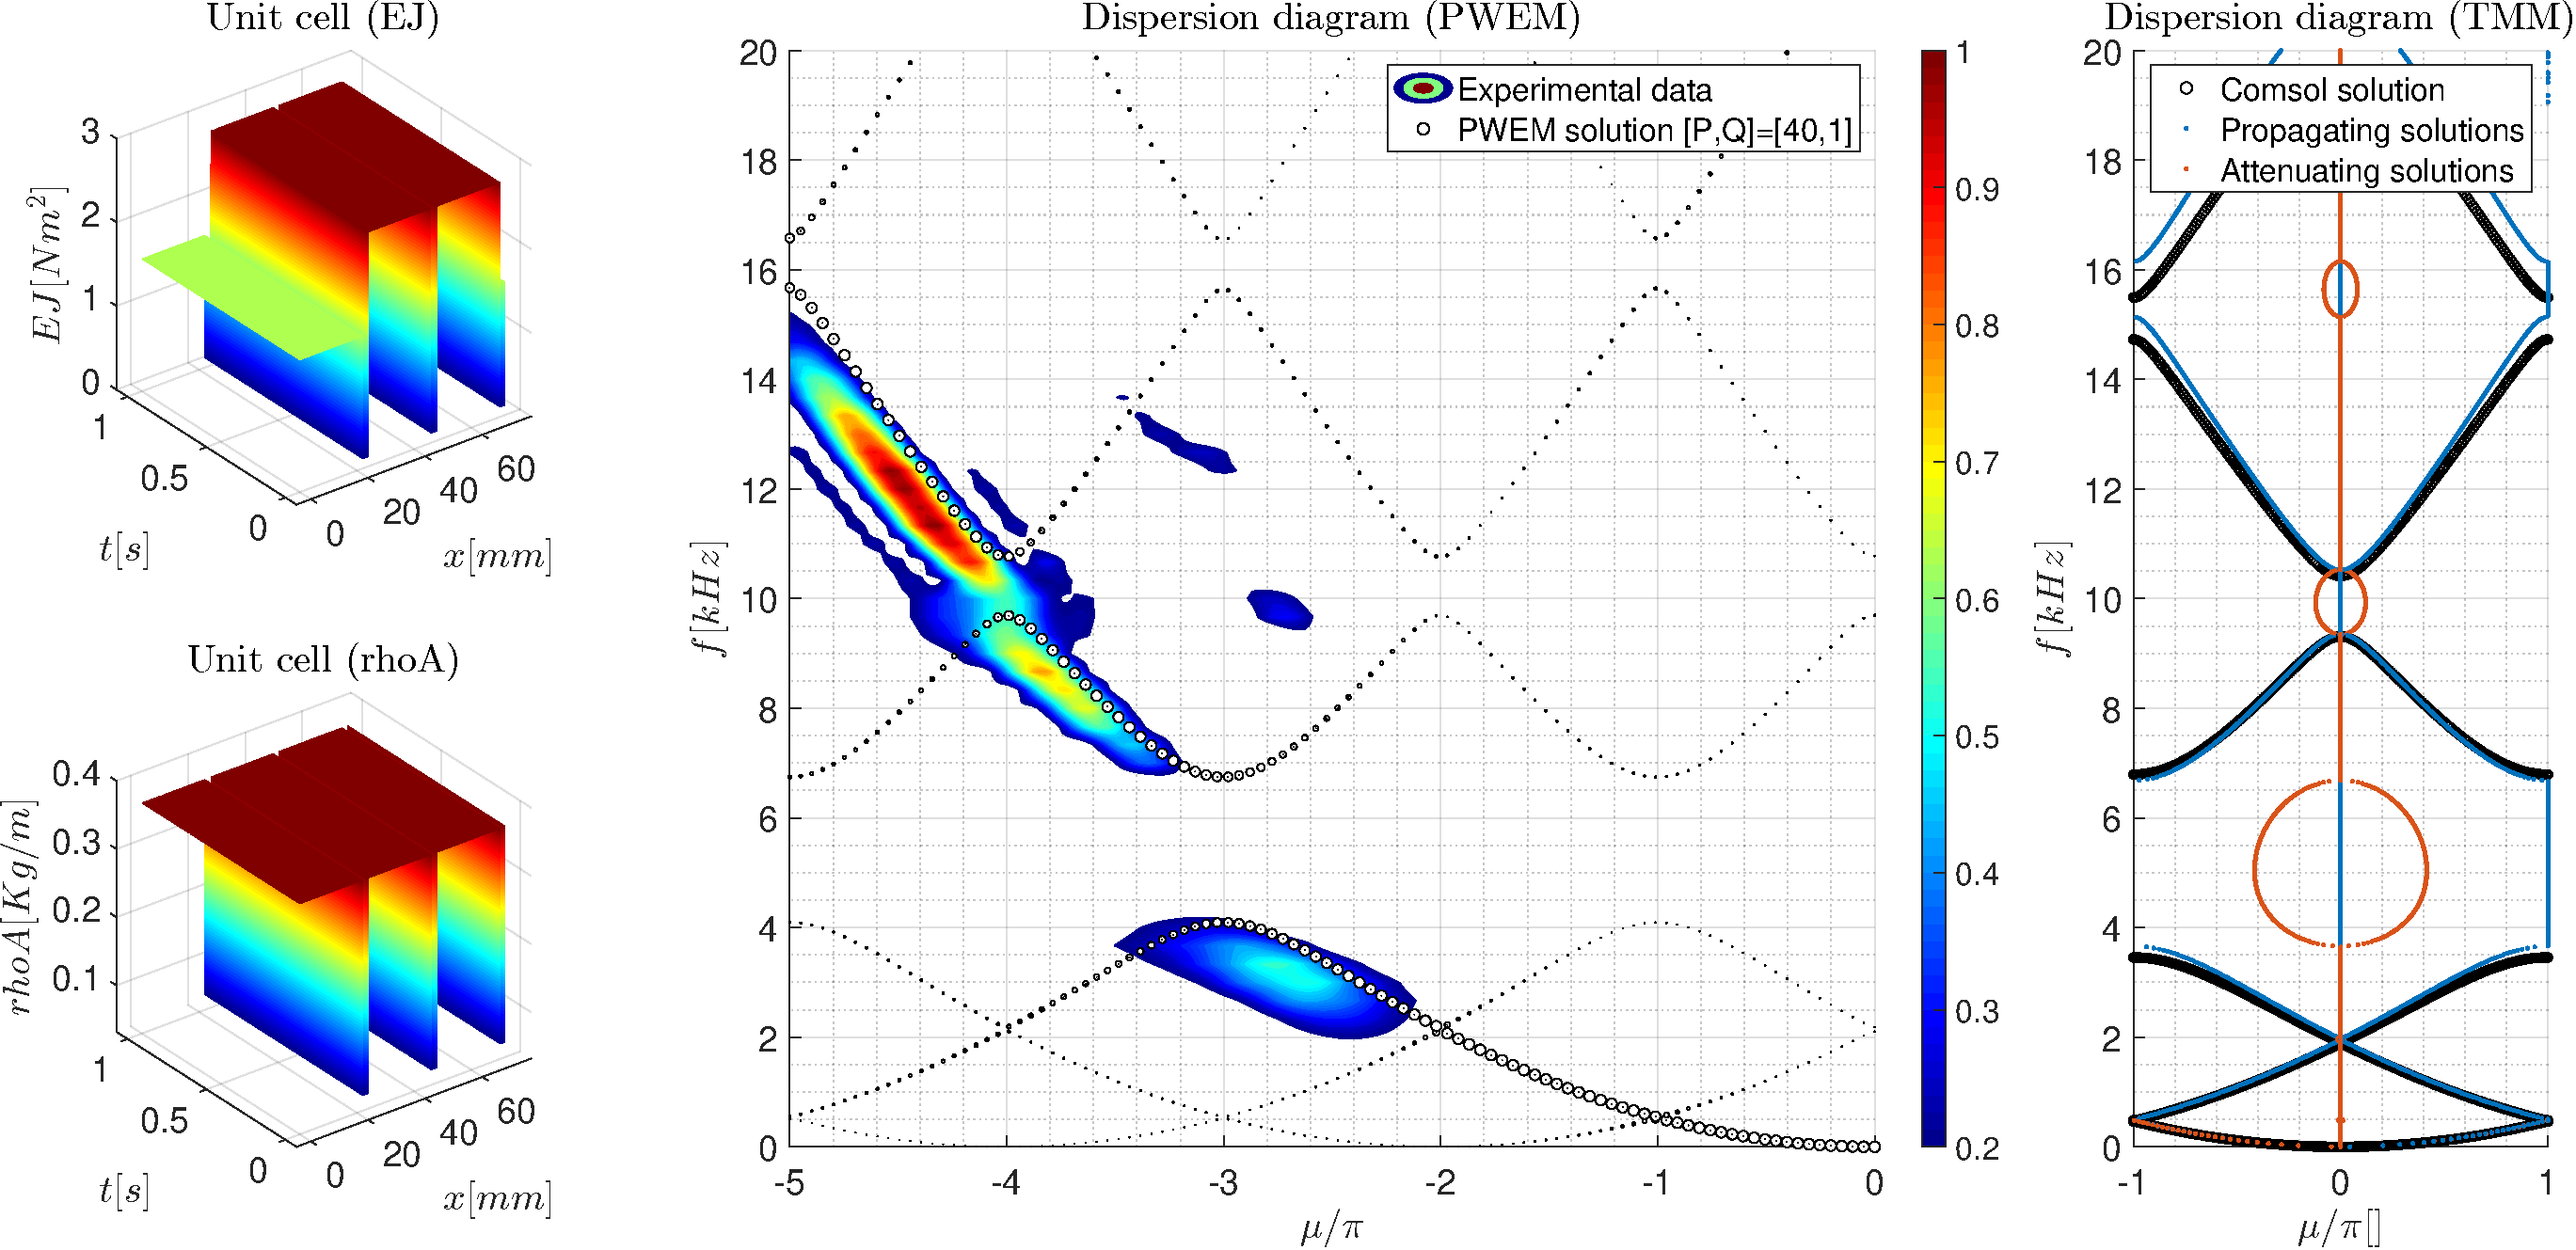
\includegraphics[width=\textwidth]{./img/MATLAB/PWEM_TMM_EXP ON-OFF-OFF @0kHz.pdf}
        \caption{Dispersion diagram for the ON-OFF-OFF configuration.}
    \end{figure}

\end{frame}



\subsection{Space-Time modulation}

\begin{frame}{Space-Time modulation}

    \begin{columns}[c, onlytextwidth]

        \begin{column}{0.55\textwidth}

            For the case of space-time modulations, piezoelectric patches are driven by equal (but phase-shifted) signals.
            Three different pairs of shunt modulation frequencies ($\pm f_m$) are considered.

            \vspace{9pt}

            PWEM numerical simulations are compared against experimental data.

        \end{column}

        \begin{column}{0.45\textwidth}

            \begin{figure}[H]
                \centering
                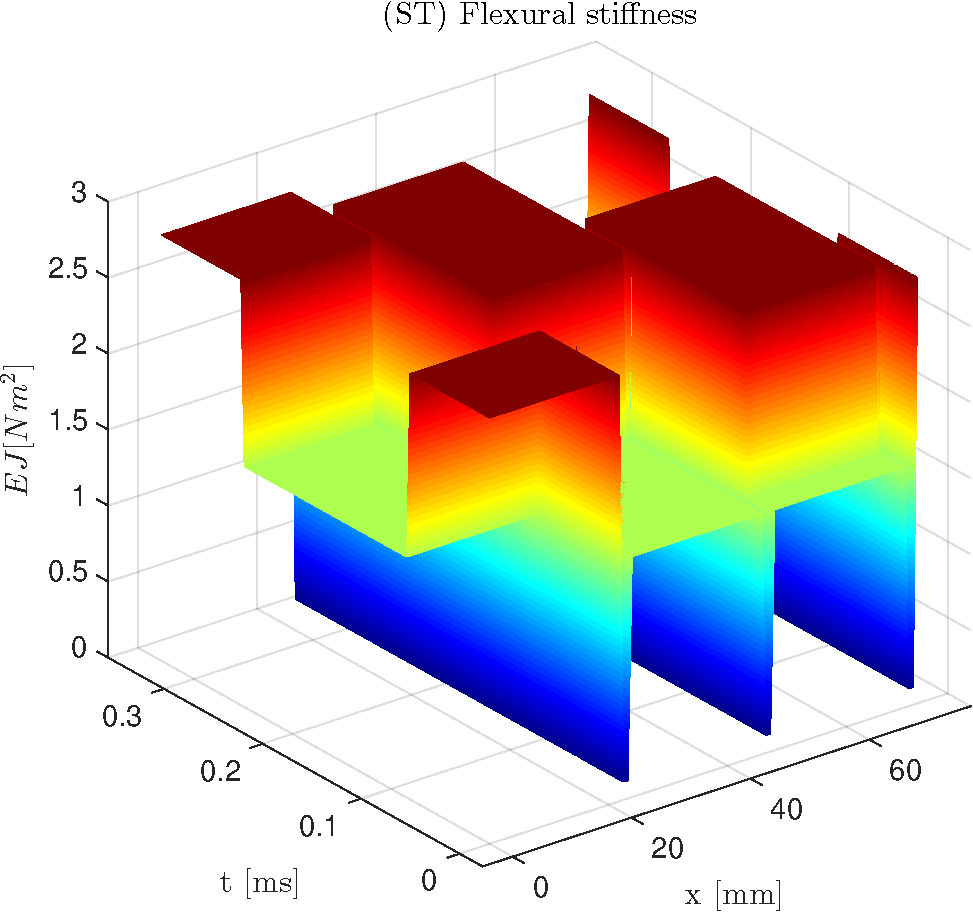
\includegraphics[width=0.9\textwidth]{img/MATLAB/ST_cell_Sinusoidal (discrete) @3kHz.pdf}
                \caption{ST cell in the case $f_m = 3 [Khz]$.}
            \end{figure}

        \end{column}

    \end{columns}

    The mechanical admittance of the $k$-th piezoelectric patch in the ST cell is given by:

    \begin{equation}
        Y_k^{SU} = \frac{(Y^{OFF} + Y^{ON})}{2} + \frac{(Y^{OFF} - Y^{ON})}{2} sign \left[ \cos \left( 2 \pi f_m t + (k-1) \frac{2\pi}{3} \right) \right]
    \end{equation}

\end{frame}



\begin{frame}{Modulation $f_m = \pm 1kHz$}


    Time modulation causes anti-symmetric dispersion diagrams and directional band-gaps to appear.
    This is a clear indication of the nonreciprocal behavior of the structure.

    A low frequency global band-gap is still present, associated with spatial modulation.

    \begin{figure}[H]
        \centering
        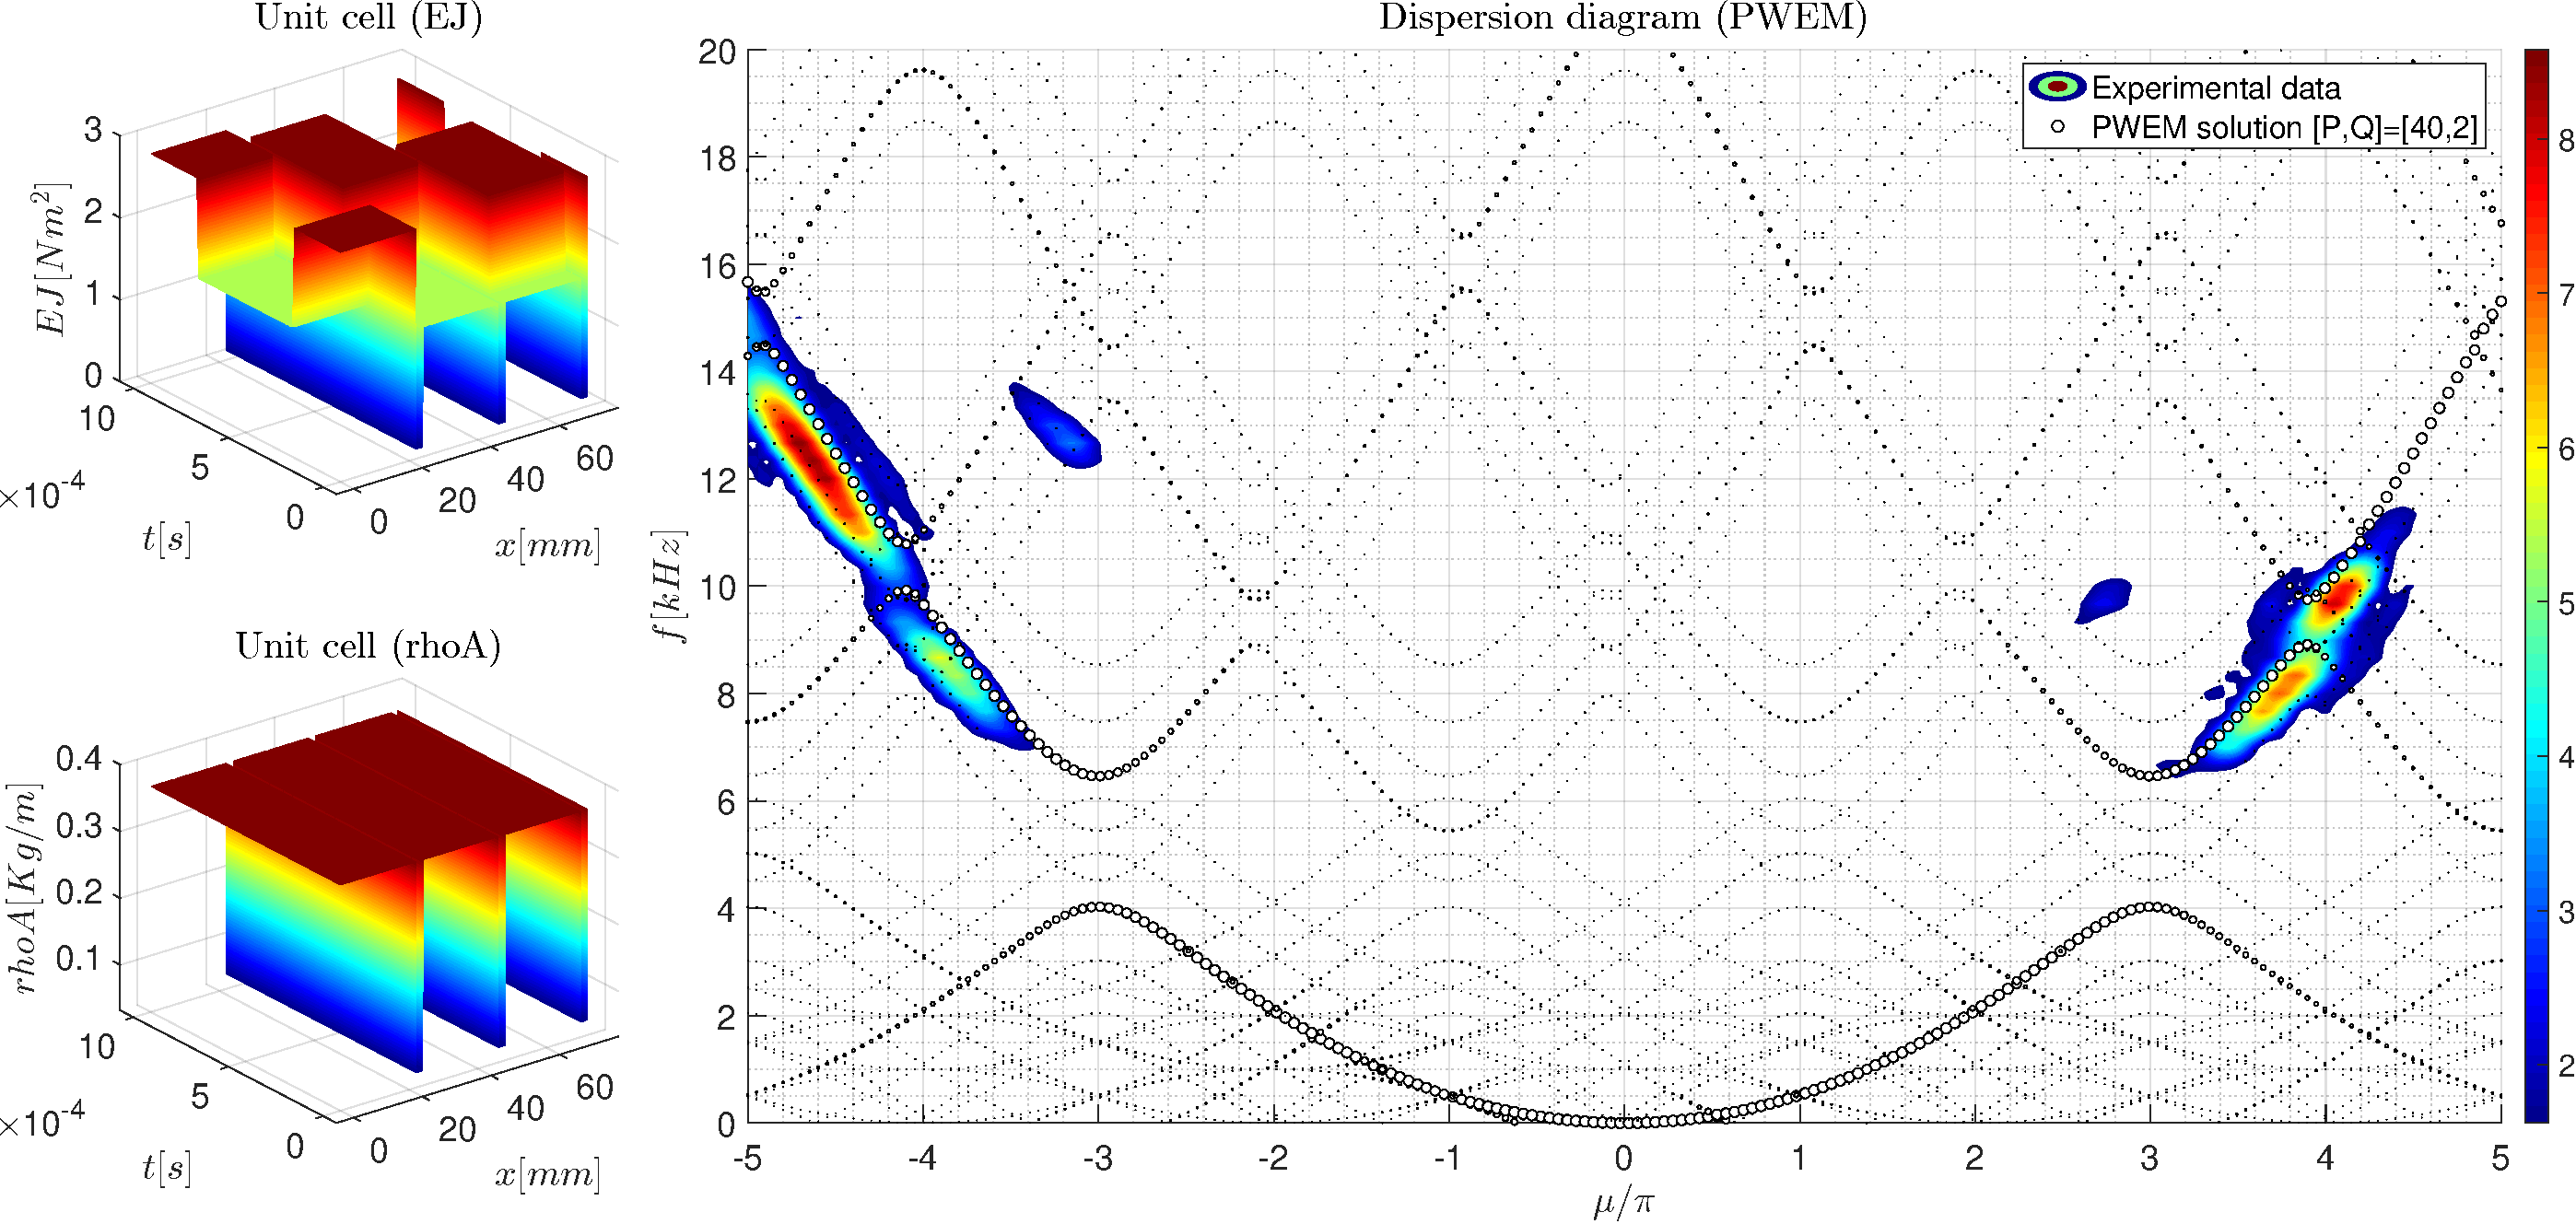
\includegraphics[width=\textwidth]{img/MATLAB/PWEM_EXP Sinusoidal (discrete) @1kHz.pdf}
        \caption{Dispersion diagram for the case of modulation frequency $f_m = \pm 1 kHz$.}
    \end{figure}

\end{frame}



\begin{frame}{Modulation $f_m = \pm 2kHz$}

    Intuitively, the phenomenon associated with the nonreciprocal behavior is now more pronounced, as the modulation frequency is doubled.
    Band-gap associated with space modulation seems to remain unchanged.

    \begin{figure}[H]
        \centering
        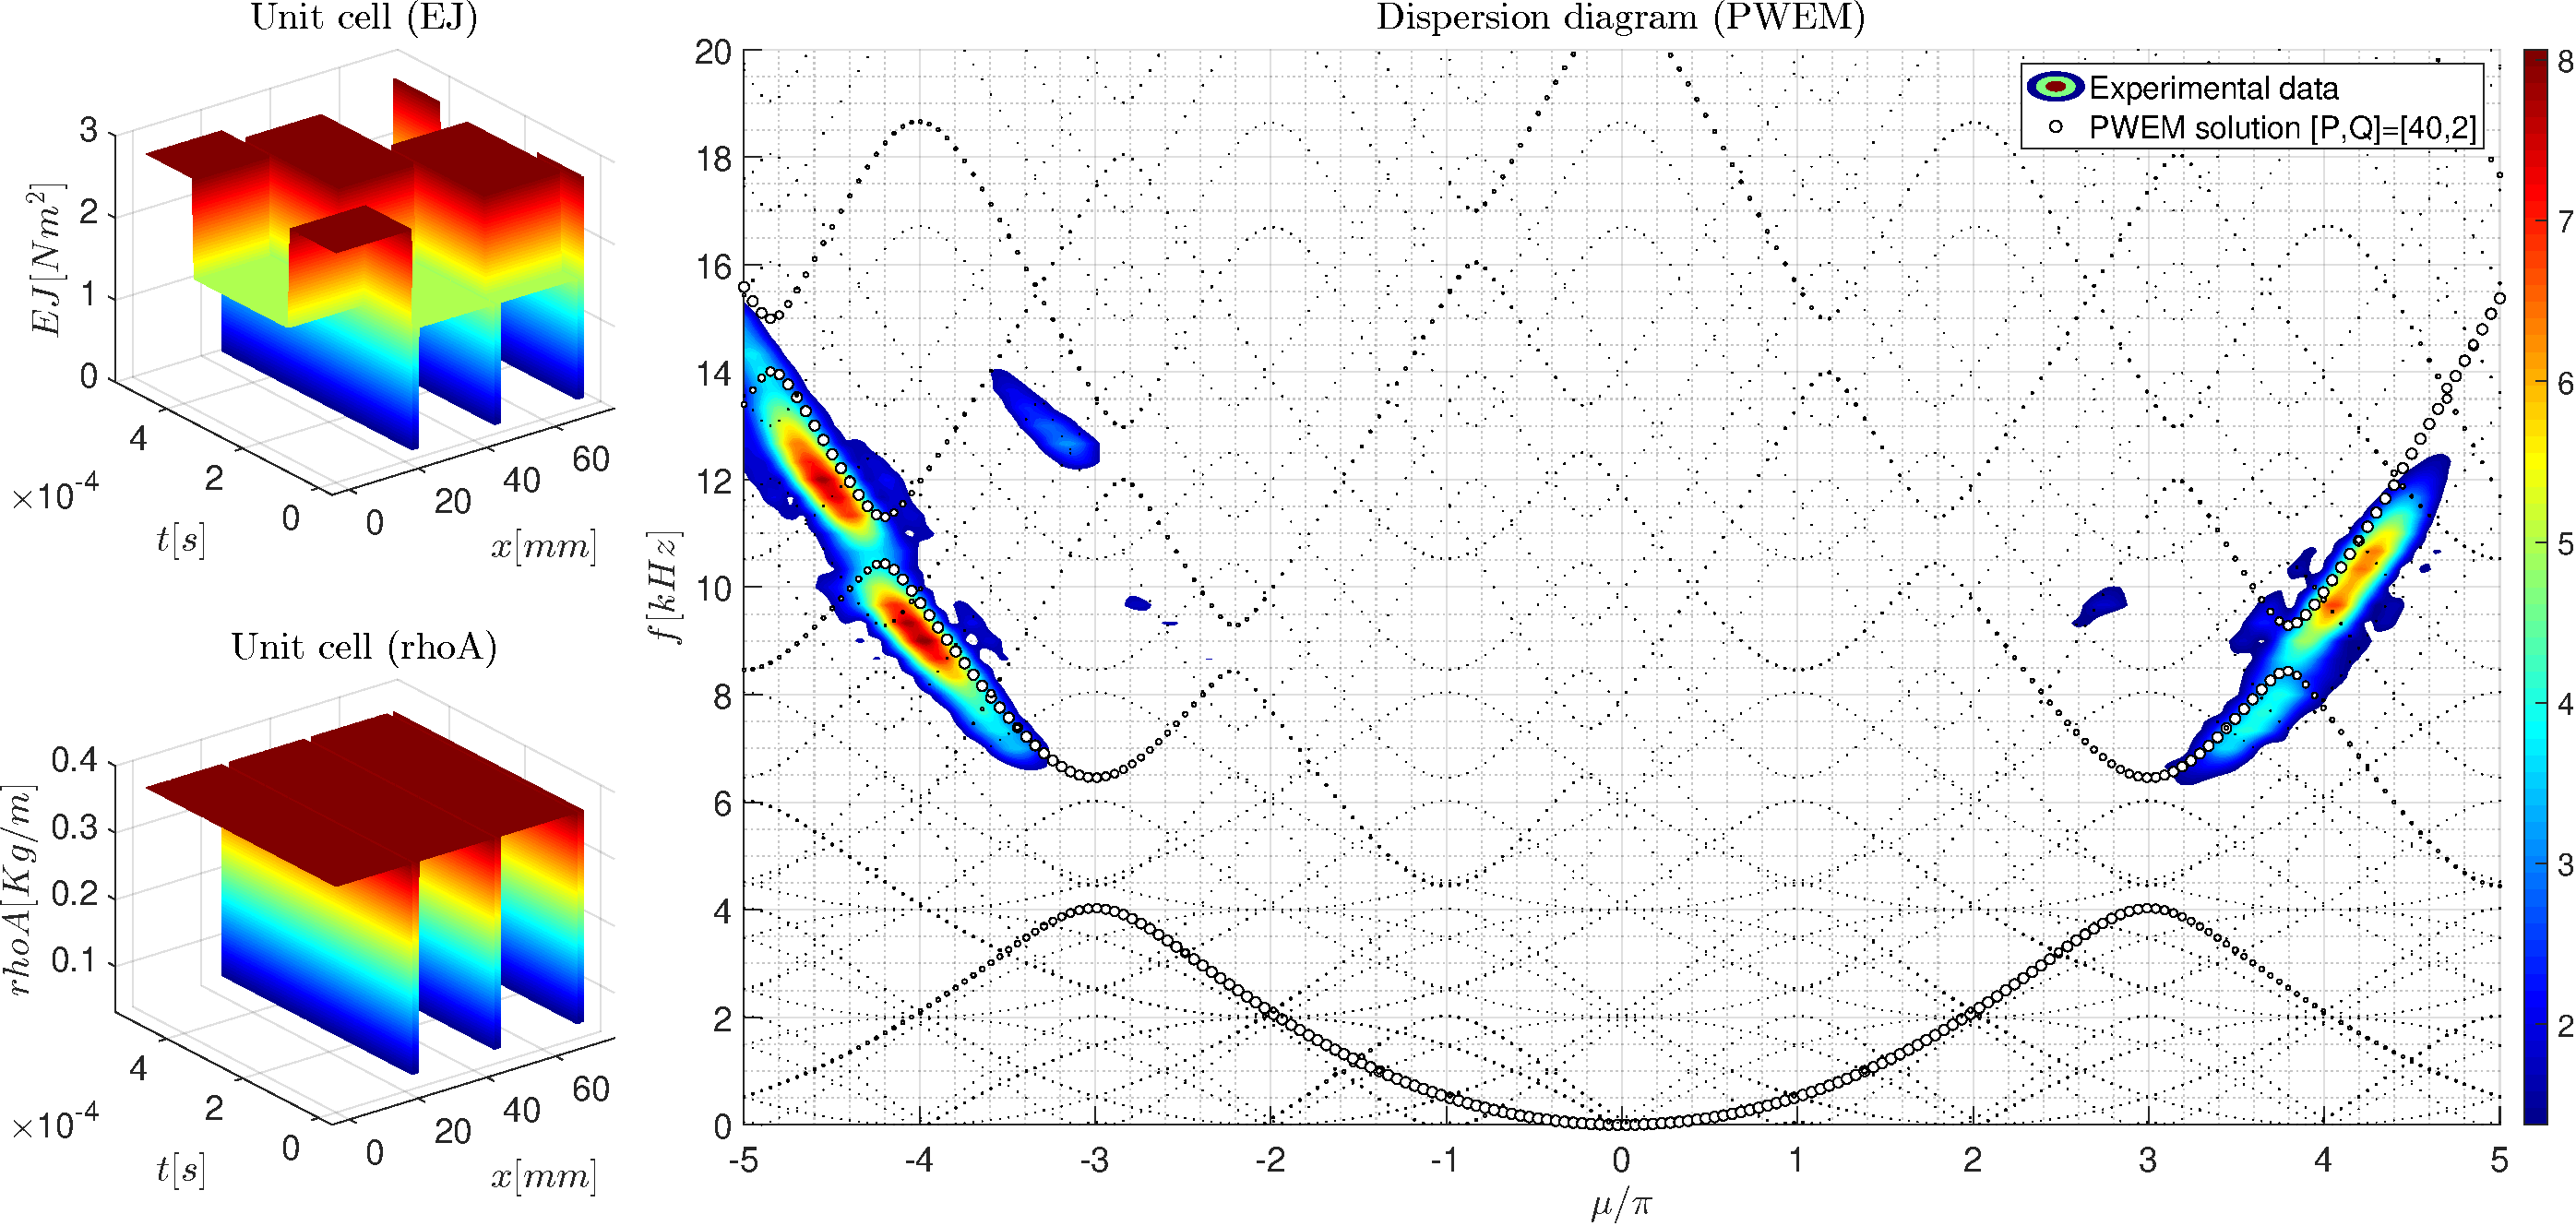
\includegraphics[width=\textwidth]{img/MATLAB/PWEM_EXP Sinusoidal (discrete) @2kHz.pdf}
        \caption{Dispersion diagram for the case of modulation frequency $f_m = \pm 2 kHz$.}
    \end{figure}


\end{frame}



\begin{frame}{Modulation $f_m = \pm 3kHz$}

    The asymmetrical shift of the already previously analyzed directional band-gaps is even more evident.
    With respect to the case $f_m = 0 kHz$ (\textit{ON-OFF-OFF}), a total shift of around $\pm1.5 kHz$ has been observed in the directional band-gaps positions.

    \begin{figure}[H]
        \centering
        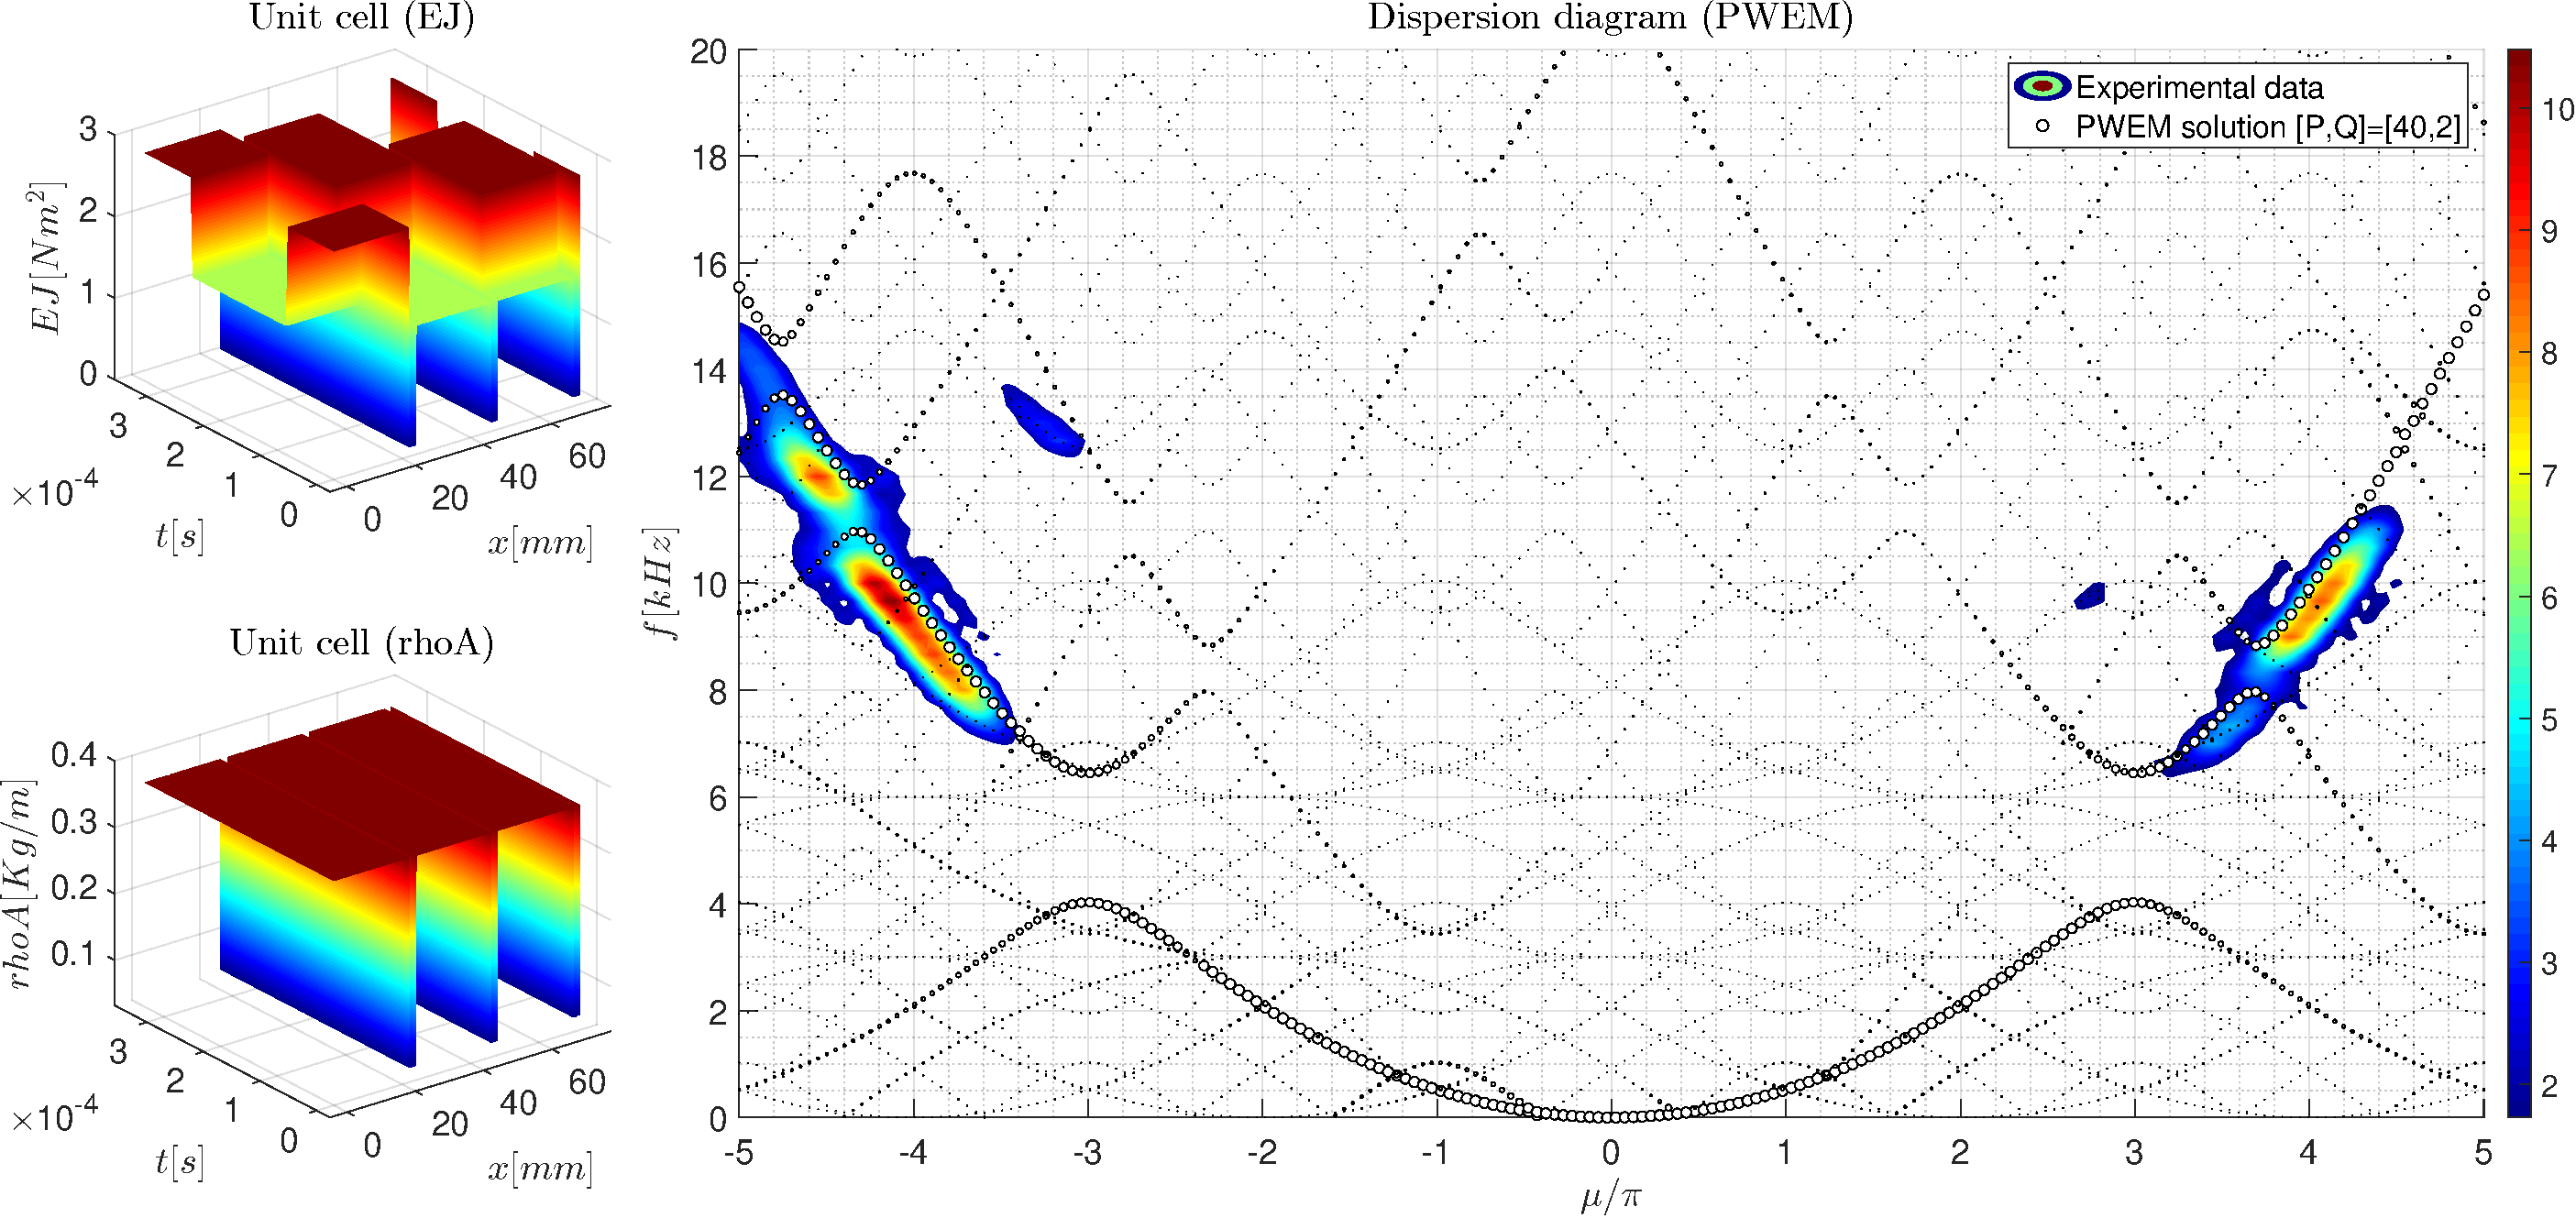
\includegraphics[width=\textwidth]{img/MATLAB/PWEM_EXP Sinusoidal (discrete) @3kHz.pdf}
        \caption{Dispersion diagram for the case of modulation frequency $f_m = \pm 3 kHz$.}
    \end{figure}

\end{frame}
\section{Nonreciprocal behavior}

\begin{frame}{Performed tests}

    Both experimental and numerical simulations have shown that the structure exhibits a nonreciprocal behavior when excited with a time-space modulated signal.

    \begin{figure}[H]
        \centering
        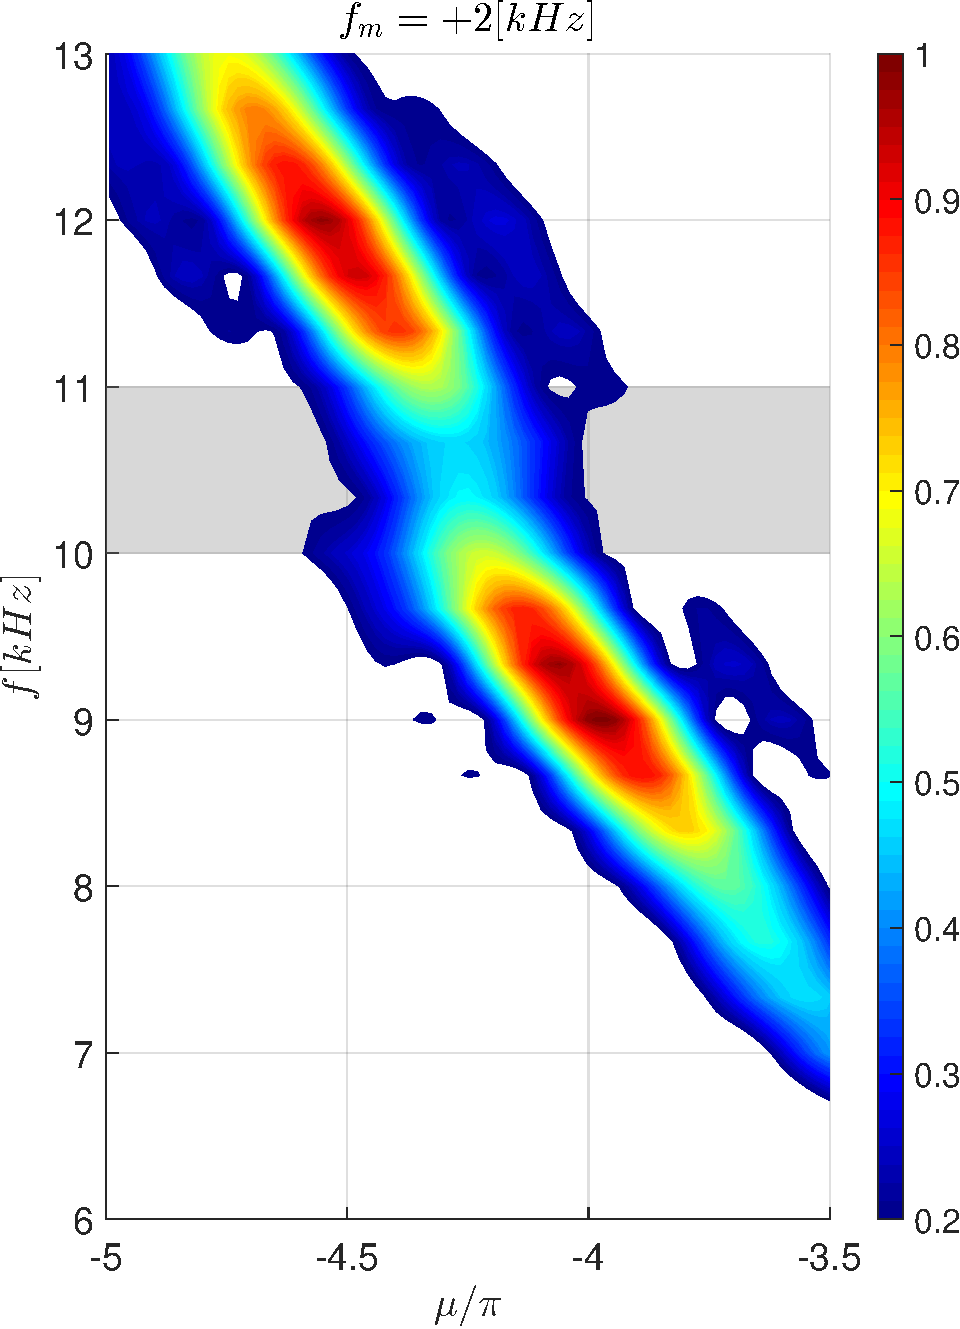
\includegraphics[width=0.3\textwidth]{img/MATLAB/EXP_nonreciprocal_@+2kHz.pdf}
        \hspace{1cm}
        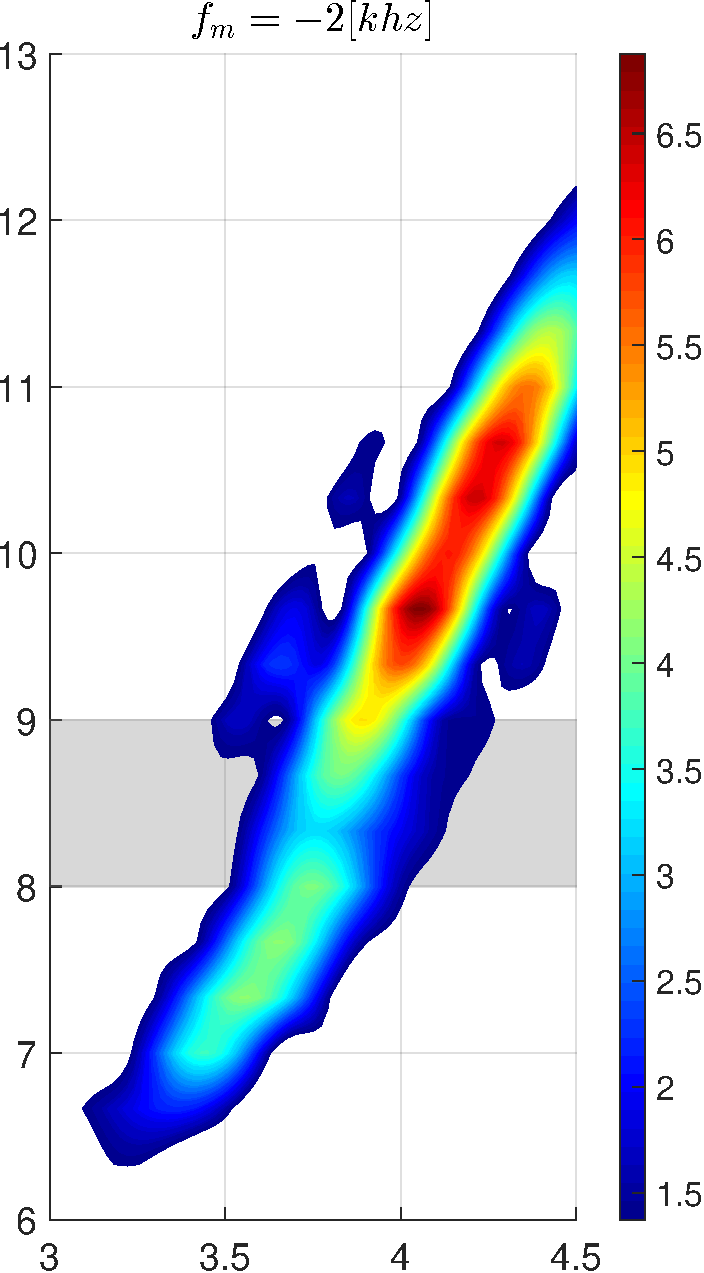
\includegraphics[width=0.3\textwidth]{img/MATLAB/EXP_nonreciprocal_@-2kHz.pdf}
        \caption{Experimental results for modulation frequency $f_m = \pm 2 kHz$.}
    \end{figure}

    Two additional tests are performed using a narrow-band excitation signal at the two directional band-gaps frequencies already identified.
    Spectral analysis of the travelling waves is performed to further highlight nonreciprocity in the structure.

\end{frame}



\begin{frame}{Spectral analysis}

    \begin{figure}[H]
        \centering
        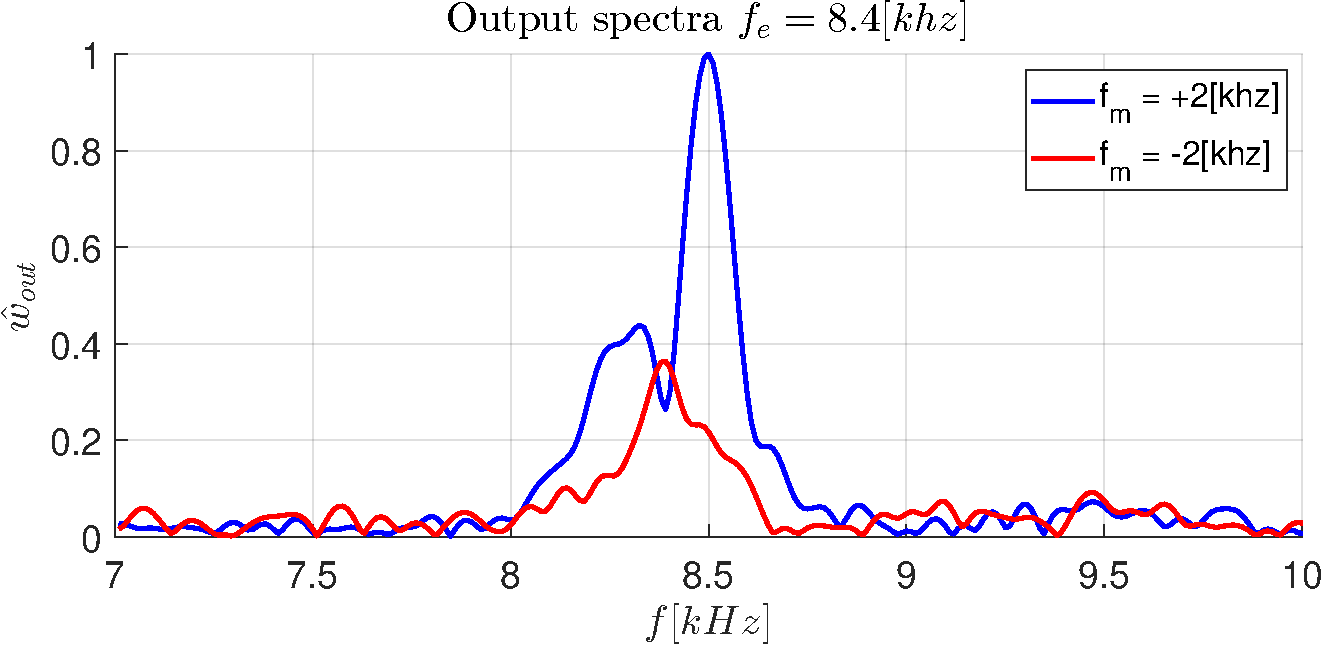
\includegraphics[width=0.49\textwidth]{img/MATLAB/Spectra_narrow8p4kHz_2000.pdf}
        \hfill
        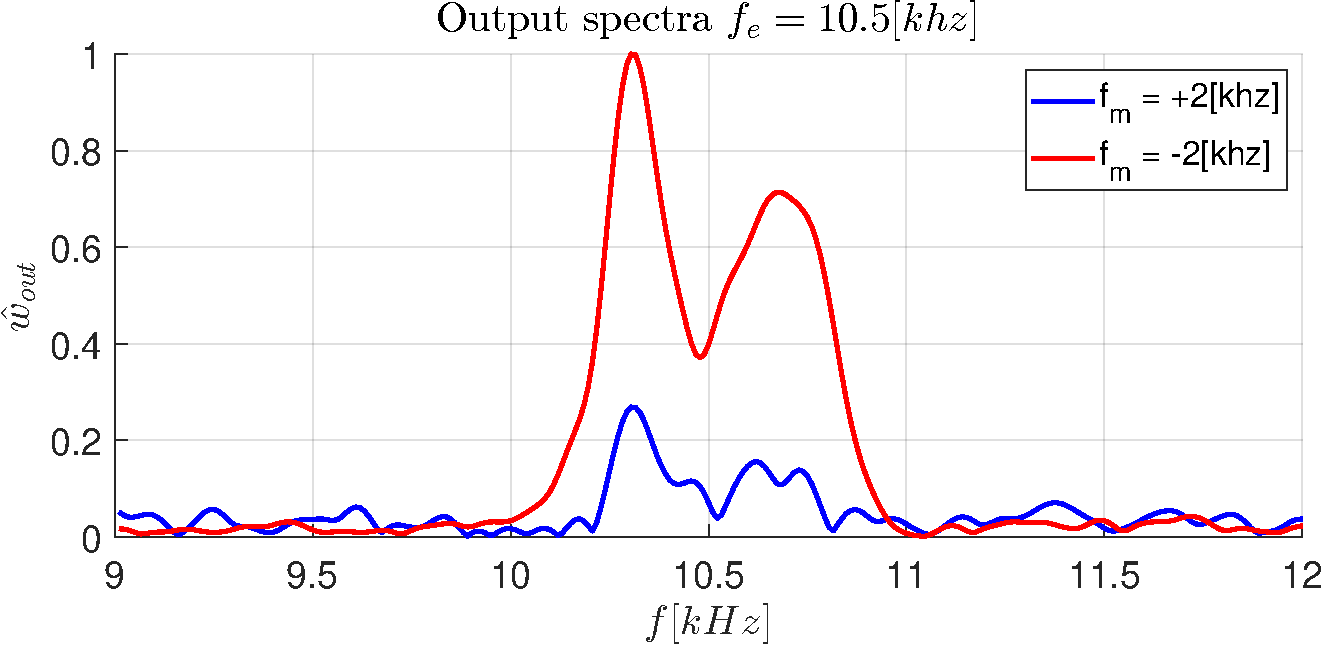
\includegraphics[width=0.49\textwidth]{img/MATLAB/Spectra_narrow10p5kHz_2000.pdf}
        \caption{Spectral components of end-of-beam displacement for (left) $f_e = 8.4 kHz$ and (right) $f_e = 10.5 kHz$ excitations. Modulation frequency is set to $f_m = \pm 2 kHz$.}
    \end{figure}

    \textbf{Depending on the travelling direction considered, the wave propagates differently.}
    The principle of reciprocity is therefore violated.

\end{frame}
\section{Conclusions}

\begin{frame}{Summary of results}

    In this work we have shown that in a 1D beam structure, \textbf{nonreciprocal behavior can be achieved and controlled} by modulating its properties in time and space via shunted piezoelectric actuation.

    \vspace{9pt}

    \textbf{The result is a diode-like behavior in the wave transmission}, where the wave is allowed to propagate in one direction while being attenuated in the opposite direction if a directional band-gap is present.

\end{frame}



\begin{frame}{Applications \& Future work}

    The capability to control wave propagation in a nonreciprocal manner opens up a wide range of potential applications in the field of phononic devices and advanced signal processing, such as:

    \begin{itemize}
        \item Acoustic waveguides for unidirectional energy transfer;
        \item Enhanced vibration control systems in engineering structures;
        \item Phononic devices for advanced signal processing.
    \end{itemize}

    \vspace{9pt}

    Future work may focus on refining the modulation strategies to achieve even greater control over wave propagation and exploring the scalability of this approach to other multidimensional structures such as plates and shells.

\end{frame}


\appendix

\begin{frame}[allowframebreaks]{References}
    \nocite{*}
    \bibliography{bibliography}
\end{frame}

\begin{frame}[standout]
    Questions?
\end{frame}

\begin{frame}[standout]
    Thank you!
\end{frame}

\end{document}